\documentclass[12pt,a4paper]{article}

% Essential packages
\usepackage[utf8]{inputenc}
\usepackage[T1]{fontenc}
\usepackage{amsmath,amssymb,amsfonts}
\usepackage{graphicx}
\usepackage{float}
\usepackage[margin=1in]{geometry}
\usepackage{hyperref}
\usepackage{fancyhdr}
\usepackage{tikz}
\usepackage{pgfplots}
\pgfplotsset{compat=1.17}
\usepackage{tcolorbox}
\usepackage{booktabs}
\usepackage{enumitem}
\usepackage{xcolor}

% Fix header height
\setlength{\headheight}{14.5pt}

% Color definitions
\definecolor{conceptblue}{RGB}{230,240,255}
\definecolor{exampleorange}{RGB}{255,245,230}
\definecolor{importantred}{RGB}{255,235,235}
\definecolor{deepgreen}{RGB}{220,245,220}
\definecolor{mathpurple}{RGB}{245,235,255}

% Custom environments
\newtcolorbox{conceptbox}[1][]{
    colback=conceptblue,
    colframe=blue!60!black,
    title=#1,
    fonttitle=\bfseries,
    boxrule=0.5pt,
    arc=3pt
}

\newtcolorbox{examplebox}[1][]{
    colback=exampleorange,
    colframe=orange!80!black,
    title=#1,
    fonttitle=\bfseries,
    boxrule=0.5pt,
    arc=3pt
}

\newtcolorbox{importantbox}{
    colback=importantred,
    colframe=red!70!black,
    boxrule=0.5pt,
    arc=3pt
}

\newtcolorbox{deepexplanation}{
    colback=deepgreen,
    colframe=green!50!black,
    boxrule=1pt,
    arc=4pt,
    left=8pt,
    right=8pt,
    top=8pt,
    bottom=8pt
}

\newtcolorbox{mathbox}{
    colback=mathpurple,
    colframe=purple!60!black,
    boxrule=0.5pt,
    arc=3pt
}

% Header/Footer
\pagestyle{fancy}
\fancyhf{}
\fancyhead[L]{Chapter 1: Introduction}
\fancyhead[R]{Digital Image Processing}
\fancyfoot[C]{\thepage}

\title{\textbf{Chapter 1: Introduction to Digital Image Processing}\\
\Large Comprehensive Study Notes with Deep Technical Analysis\\
\normalsize Based on Gonzalez \& Woods (3rd Edition) and CPE415 Lectures}
\author{Study Notes with Deep Technical Explanations}
\date{Spring 2026}

\begin{document}

\maketitle
\tableofcontents
\newpage

%==============================================================================
\section{What is Digital Image Processing?}
%==============================================================================

\begin{conceptbox}[Definition of a Digital Image]
A \textbf{digital image} is a two-dimensional function $f(x, y)$ where:
\begin{itemize}
    \item $(x, y)$ are \textbf{spatial coordinates}
    \item $f(x, y)$ is the \textbf{intensity} (or gray level) at that point
    \item When $x$, $y$, and $f$ are all \textbf{finite, discrete quantities}, we have a digital image
\end{itemize}

\textbf{Digital Image Processing} refers to processing digital images by means of a digital computer.
\end{conceptbox}

\subsection{The Origins: Why Process Images?}

Digital image processing has its origins in two principal application areas:
\begin{enumerate}
    \item \textbf{Improvement of pictorial information} for human interpretation
    \item \textbf{Processing of image data} for storage, transmission, and representation for autonomous machine perception
\end{enumerate}

\subsection{The First Digital Image}

\begin{figure}[H]
    \centering
    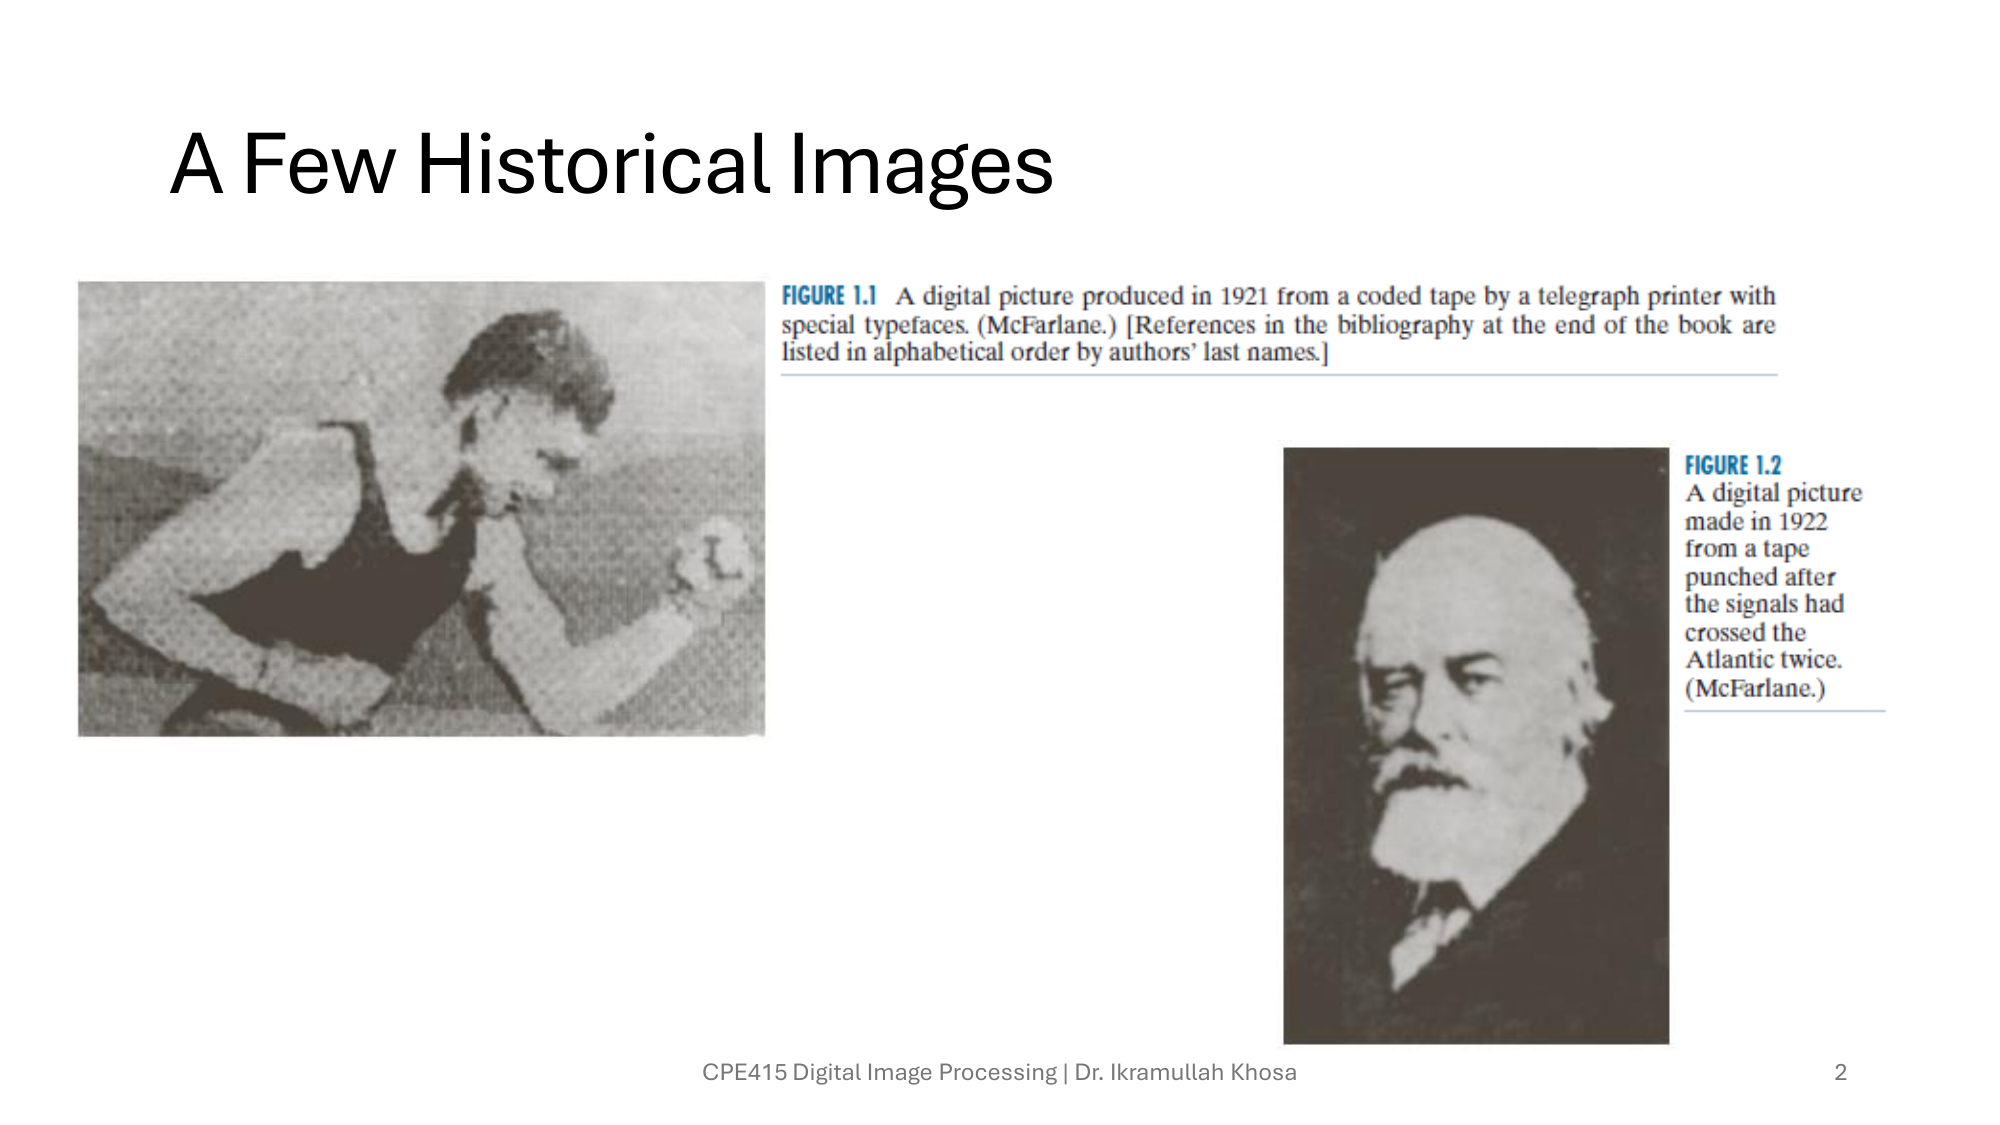
\includegraphics[width=0.85\textwidth]{images/slide1-02.png}
    \caption{Historical images in digital image processing}
    \label{fig:historical1}
\end{figure}

\begin{deepexplanation}
\textbf{DEEP ANALYSIS - Figure \ref{fig:historical1}: The Birth of Digital Imaging}

\textbf{Historical Context:}
The first digital image was transmitted via submarine cable between London and New York in 1921 using the Bartlane cable picture transmission system. This system reduced the time required to transport a picture across the Atlantic from more than a week to less than three hours.

\textbf{Technical Details of Early Systems:}
\begin{itemize}
    \item Early systems used \textbf{5 distinct gray levels} (coded for transmission)
    \item By 1929, systems could use \textbf{15 gray levels}
    \item Images were printed on a telegraph printer with special typefaces
    \item Resolution was limited by the printing mechanism
\end{itemize}

\textbf{Key Milestone:}
The first photograph scanned into a digital computer was made in 1957 at the US National Bureau of Standards. This 176×176 pixel image of a son of Russell Kirsch is considered the first truly digital image.

\textbf{Why This Matters:}
\begin{itemize}
    \item Demonstrated that images could be \textbf{encoded numerically}
    \item Showed that \textbf{quantized} representations could be useful
    \item Led to development of image compression and transmission
    \item Foundation for all modern digital photography and imaging
\end{itemize}
\end{deepexplanation}

\begin{figure}[H]
    \centering
    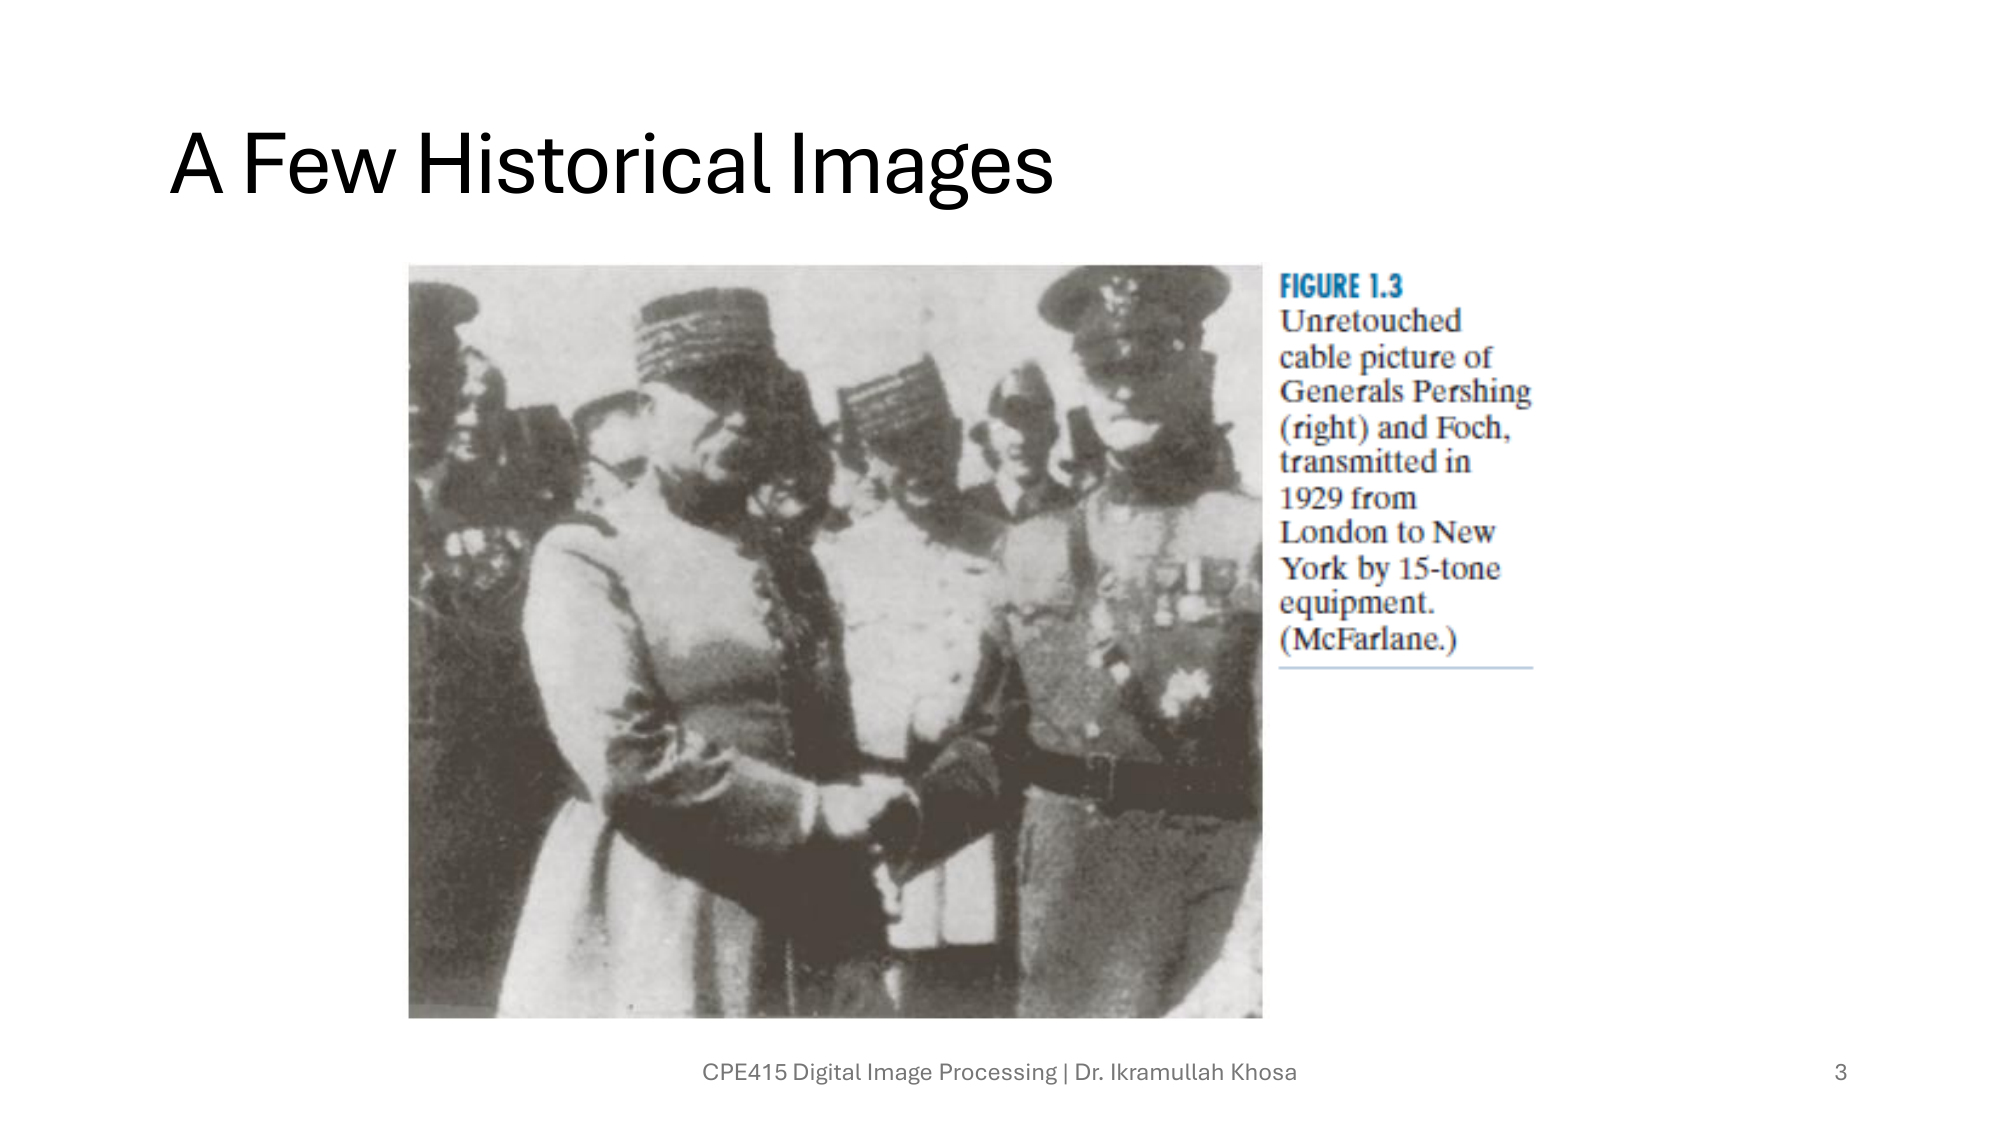
\includegraphics[width=0.85\textwidth]{images/slide1-03.png}
    \caption{More historical images and early image processing}
    \label{fig:historical2}
\end{figure}

\begin{deepexplanation}
\textbf{DEEP ANALYSIS - Figure \ref{fig:historical2}: Evolution of Digital Imaging}

\textbf{The Space Program Era (1960s):}
Digital image processing truly emerged with the space program:
\begin{itemize}
    \item \textbf{1964}: Ranger 7 transmitted first close-up images of the Moon
    \item Images required computer processing to correct geometric distortions from on-board camera
    \item JPL (Jet Propulsion Laboratory) pioneered image enhancement techniques
\end{itemize}

\textbf{Medical Imaging Revolution:}
\begin{itemize}
    \item \textbf{1971}: First CT (Computed Tomography) scanner by Godfrey Hounsfield
    \item CT uses X-ray projections from multiple angles + computer reconstruction
    \item Nobel Prize in 1979 for this revolutionary imaging technique
\end{itemize}

\textbf{Why Computer Processing Was Essential:}
\begin{enumerate}
    \item Raw data from sensors is often degraded (noise, distortion)
    \item Human interpretation can be aided by enhancement
    \item Automated analysis requires standardized digital representation
    \item Transmission and storage benefit from digital format
\end{enumerate}
\end{deepexplanation}

\begin{figure}[H]
    \centering
    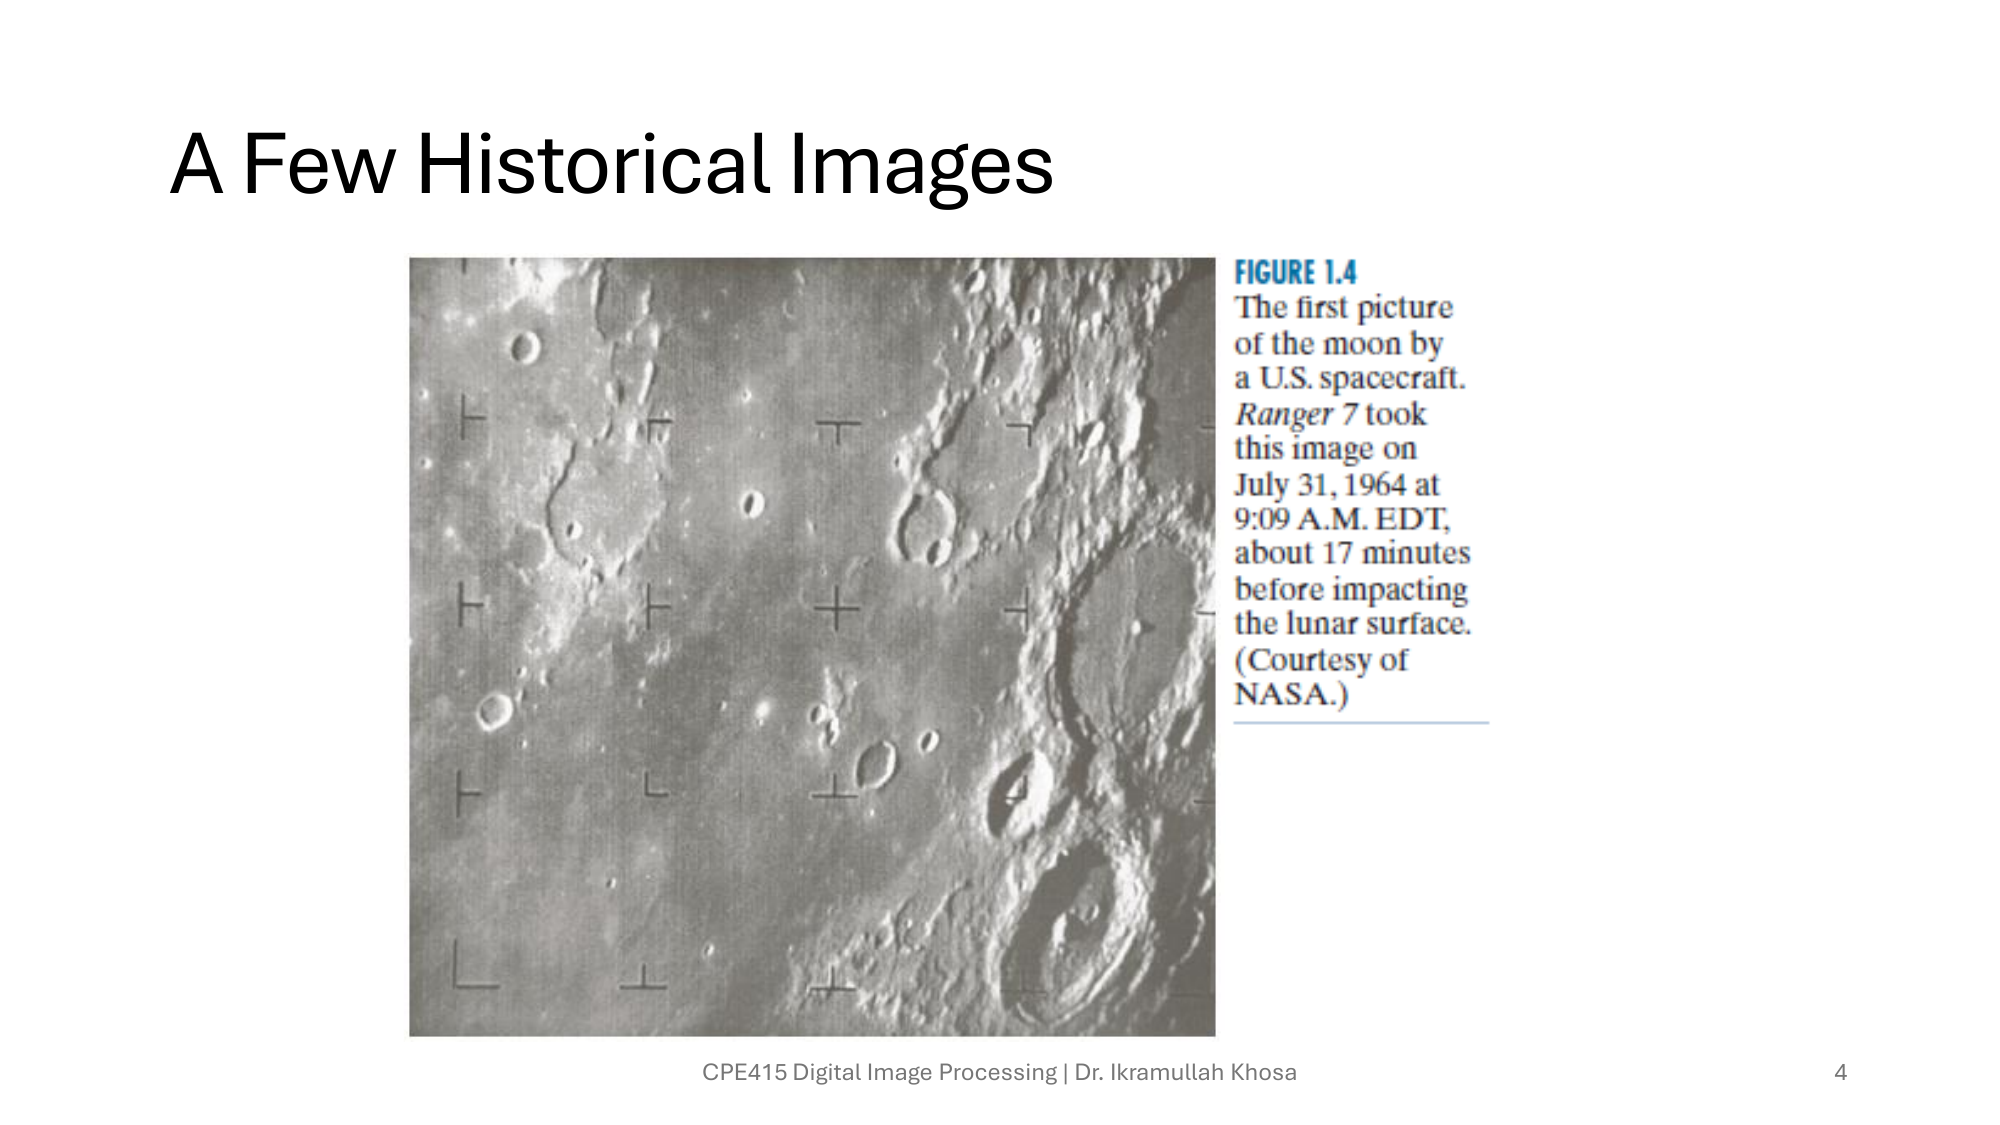
\includegraphics[width=0.85\textwidth]{images/slide1-04.png}
    \caption{Additional historical examples}
    \label{fig:historical3}
\end{figure}

%==============================================================================
\section{The Electromagnetic Spectrum}
%==============================================================================

\begin{conceptbox}[Image Formation and Energy]
All imaging systems work on the same principle:
\begin{enumerate}
    \item \textbf{Energy source} illuminates or is emitted by the scene
    \item \textbf{Sensor} captures energy reflected/transmitted/emitted by objects
    \item \textbf{Digitizer} converts analog sensor output to digital form
\end{enumerate}

The energy source determines what type of information we can capture about a scene.
\end{conceptbox}

\begin{figure}[H]
    \centering
    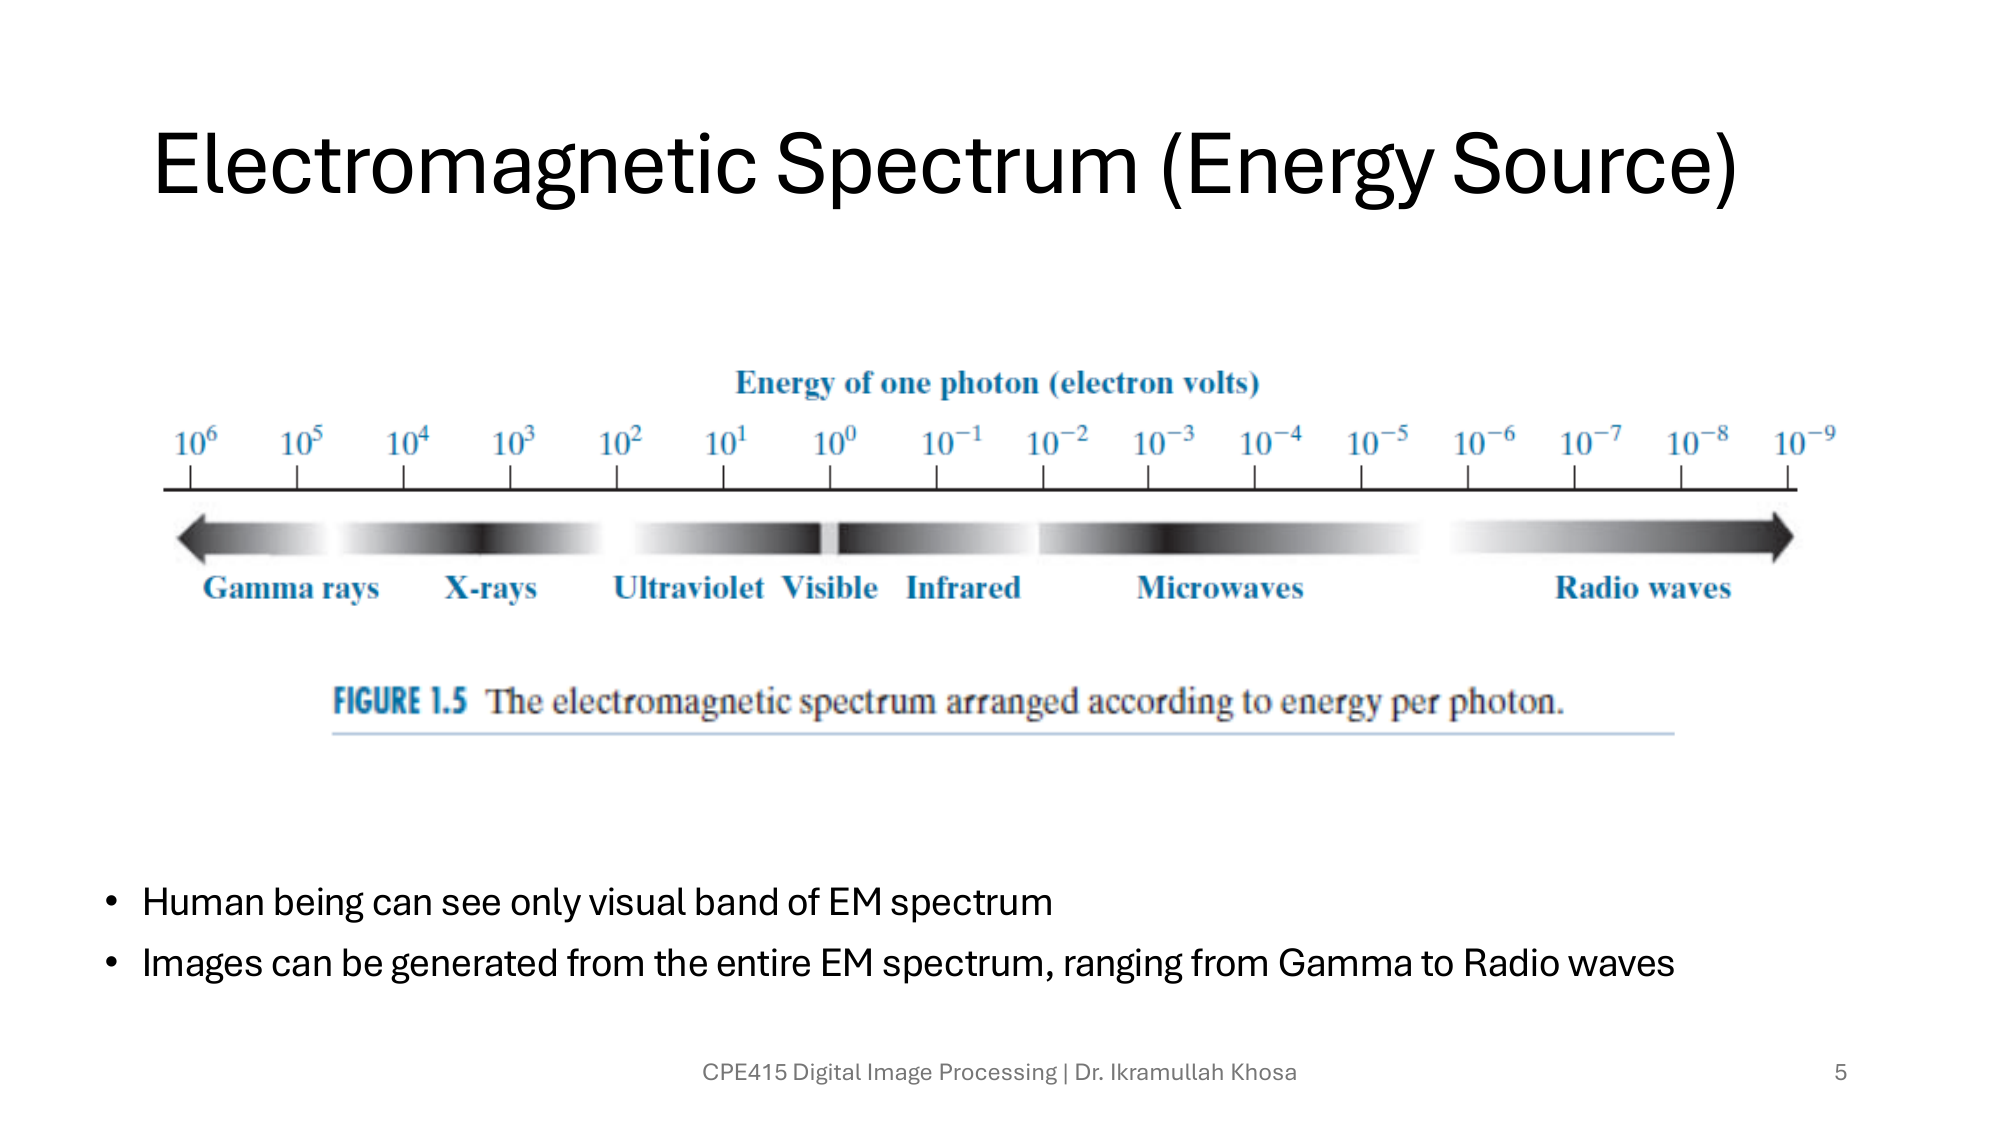
\includegraphics[width=0.95\textwidth]{images/slide1-05.png}
    \caption{The electromagnetic spectrum showing various imaging bands}
    \label{fig:em_spectrum}
\end{figure}

\begin{deepexplanation}
\textbf{DEEP ANALYSIS - Figure \ref{fig:em_spectrum}: The Full EM Spectrum for Imaging}

\textbf{What the Electromagnetic Spectrum Reveals:}
Different wavelengths of EM radiation interact differently with matter, revealing different information:

\begin{center}
\begin{tabular}{|l|l|l|l|}
\hline
\textbf{Band} & \textbf{Wavelength} & \textbf{Energy} & \textbf{What It Shows} \\
\hline
Gamma rays & $< 0.01$ nm & Highest & Nuclear processes, radioactive decay \\
X-rays & $0.01$--$10$ nm & Very high & Bone structure, dense materials \\
Ultraviolet & $10$--$400$ nm & High & Surface fluorescence, chemical \\
Visible & $400$--$700$ nm & Medium & Color, surface appearance \\
Near IR & $700$ nm--$1$ µm & Lower & Vegetation health, heat \\
Thermal IR & $3$--$15$ µm & Low & Temperature distribution \\
Microwave & $1$ mm--$1$ m & Very low & Through clouds, all-weather \\
Radio & $> 1$ m & Lowest & Deep penetration, medical MRI \\
\hline
\end{tabular}
\end{center}

\textbf{The Key Insight:}
Humans can only see the visible band (400--700 nm), which is a tiny fraction of the EM spectrum. Digital image processing allows us to ``see'' and analyze the entire spectrum!

\textbf{Physical Relationships:}
\[
c = \lambda \cdot \nu, \quad E = h\nu = \frac{hc}{\lambda}
\]
\begin{itemize}
    \item Shorter wavelength $\rightarrow$ higher frequency $\rightarrow$ higher energy
    \item Higher energy radiation can penetrate/interact with smaller structures
    \item This is why X-rays can image bones and gamma rays can detect nuclear activity
\end{itemize}
\end{deepexplanation}

%==============================================================================
\section{Imaging Across the EM Spectrum}
%==============================================================================

\subsection{Gamma Ray Imaging}

\begin{figure}[H]
    \centering
    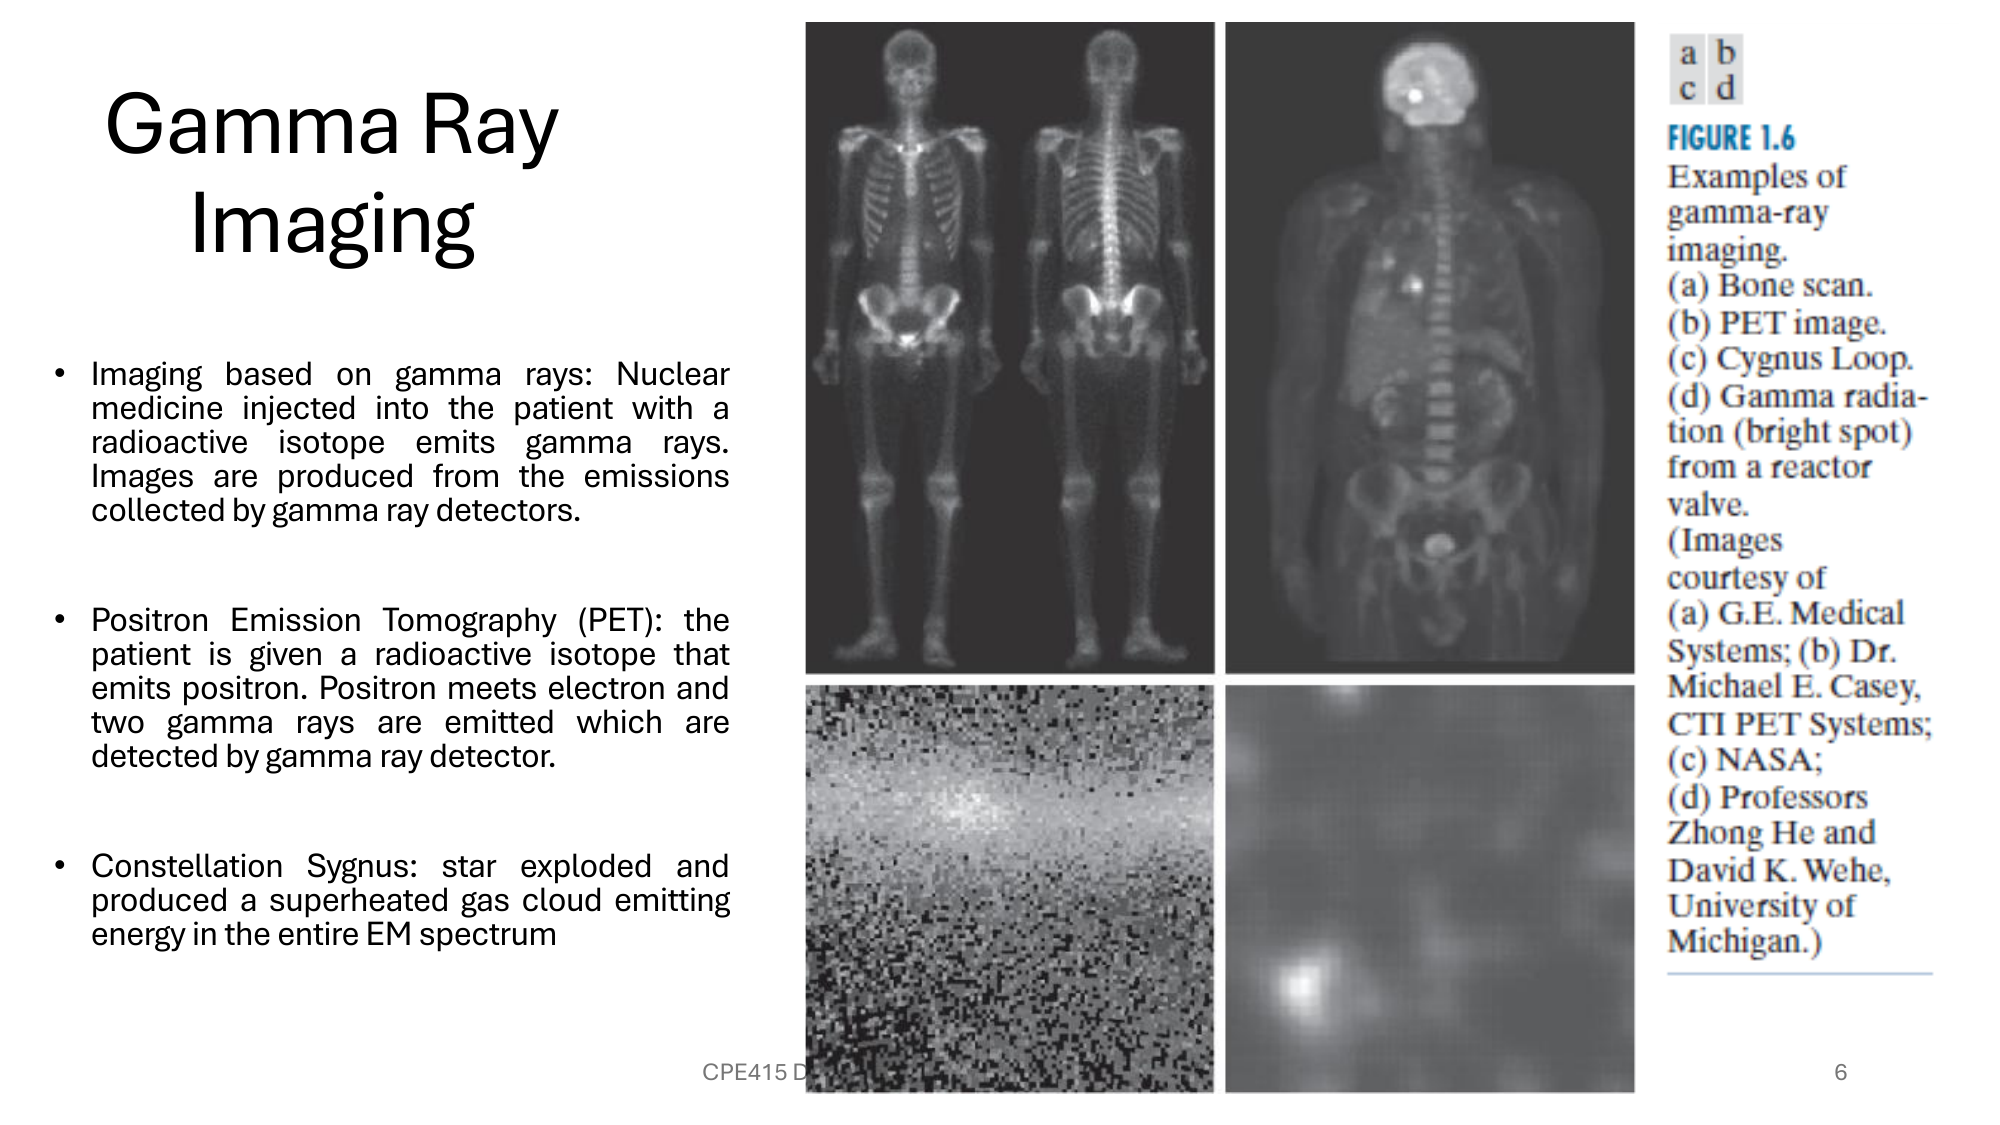
\includegraphics[width=0.9\textwidth]{images/slide1-06.png}
    \caption{Gamma ray imaging applications}
    \label{fig:gamma_imaging}
\end{figure}

\begin{deepexplanation}
\textbf{DEEP ANALYSIS - Figure \ref{fig:gamma_imaging}: Gamma Ray Imaging Explained}

\textbf{How Gamma Ray Imaging Works:}

\textbf{1. Nuclear Medicine (SPECT):}
\begin{itemize}
    \item Patient is injected with a \textbf{radioactive tracer} (radioactive isotope attached to a molecule)
    \item The tracer accumulates in target tissue (e.g., cancer cells metabolize more glucose)
    \item Gamma rays are emitted as the isotope decays
    \item A \textbf{gamma camera} detects these emissions
    \item Computer reconstructs a 3D image showing tracer distribution
\end{itemize}

\textbf{2. Positron Emission Tomography (PET):}
\begin{itemize}
    \item Uses isotopes that emit \textbf{positrons} (anti-electrons)
    \item When positron meets electron: \textbf{annihilation} occurs
    \item Two gamma rays emitted at exactly 180° apart (511 keV each)
    \item Detectors arranged in a ring around patient
    \item Coincidence detection: If two detectors fire simultaneously, the source was on the line between them
    \item Computer reconstructs image from many such lines
\end{itemize}

\textbf{3. Astronomical Gamma Imaging:}
\begin{itemize}
    \item Gamma rays from space indicate extreme events: supernovae, black holes, neutron stars
    \item Cannot be observed from ground (atmosphere absorbs)
    \item Requires space-based telescopes (e.g., Fermi Gamma-ray Space Telescope)
\end{itemize}

\textbf{Why Gamma Imaging Is Unique:}
\begin{itemize}
    \item \textbf{Functional imaging}: Shows what tissue is \textbf{doing}, not just structure
    \item Metabolically active tissue (tumors) ``lights up''
    \item Essential for cancer detection and staging
    \item Can detect disease before structural changes occur
\end{itemize}
\end{deepexplanation}

\subsection{X-Ray Imaging}

\begin{figure}[H]
    \centering
    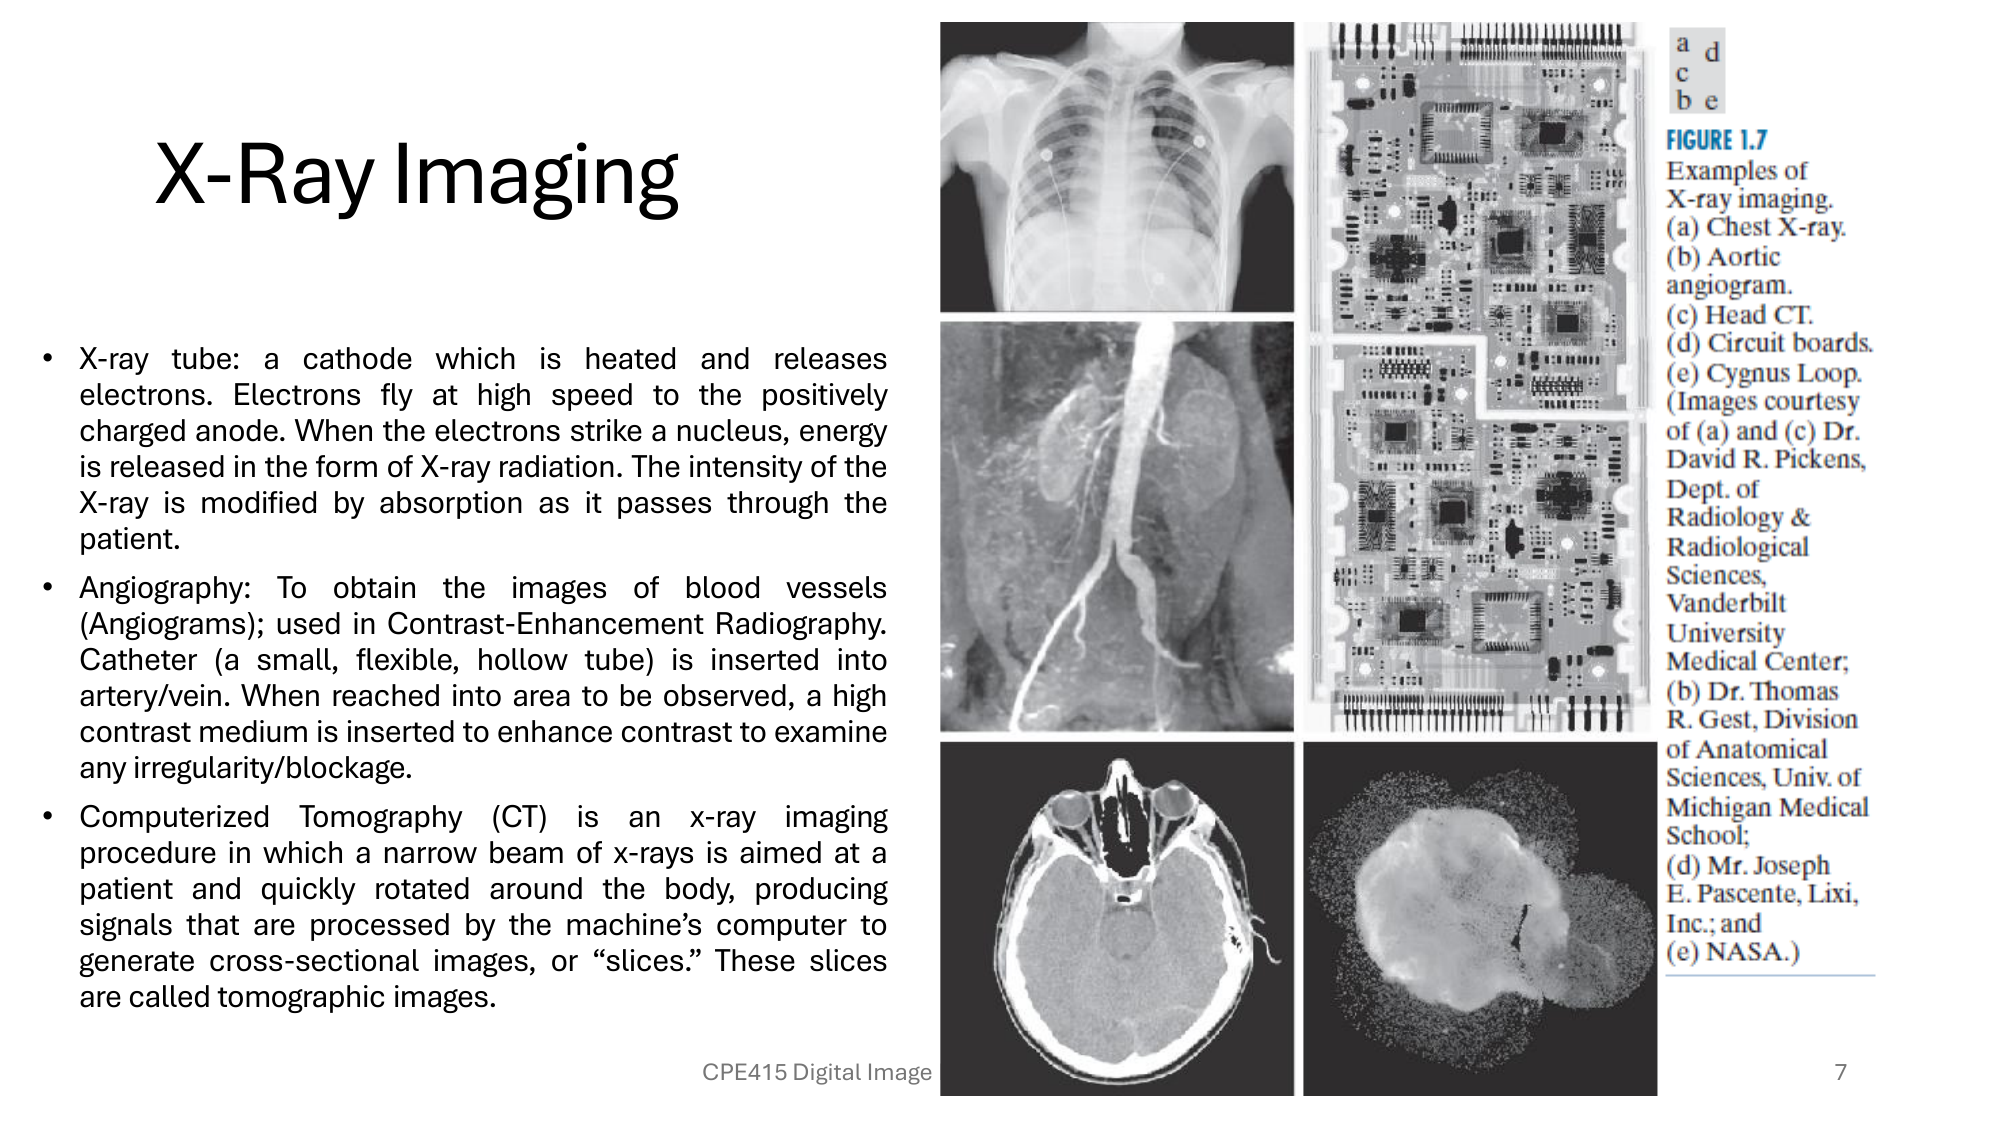
\includegraphics[width=0.9\textwidth]{images/slide1-07.png}
    \caption{X-ray imaging: standard radiography, angiography, and CT}
    \label{fig:xray_imaging}
\end{figure}

\begin{deepexplanation}
\textbf{DEEP ANALYSIS - Figure \ref{fig:xray_imaging}: X-Ray Imaging Technologies}

\textbf{How X-Rays Are Generated:}
\begin{enumerate}
    \item Cathode (heated filament) releases electrons via thermionic emission
    \item High voltage (30--150 kV) accelerates electrons toward anode
    \item Electrons strike metal target (usually tungsten)
    \item Rapid deceleration converts kinetic energy to X-ray photons
    \item Only $\approx 1\%$ of energy becomes X-rays; rest is heat
\end{enumerate}

\textbf{Image Formation:}
\begin{itemize}
    \item X-rays pass through patient
    \item Different tissues absorb different amounts (based on density and atomic number)
    \item Bone (high Ca content) absorbs strongly $\rightarrow$ appears white
    \item Air (lungs) absorbs little $\rightarrow$ appears black
    \item Soft tissue $\rightarrow$ intermediate gray levels
\end{itemize}

\textbf{Beer-Lambert Law (Attenuation):}
\[
I = I_0 e^{-\mu x}
\]
where $I_0$ = incident intensity, $\mu$ = attenuation coefficient, $x$ = thickness.

\textbf{Angiography:}
\begin{itemize}
    \item Blood vessels have similar density to surrounding tissue
    \item Inject \textbf{contrast agent} (iodine-based, high X-ray absorption)
    \item Vessels containing contrast become visible
    \item \textbf{Digital Subtraction Angiography (DSA)}: Subtract pre-contrast from post-contrast image to isolate vessels
\end{itemize}

\textbf{Computed Tomography (CT):}
\begin{itemize}
    \item Standard X-ray: 2D projection (3D$\rightarrow$2D, information loss)
    \item CT: Multiple projections at many angles around patient
    \item Computer reconstructs 3D volume using \textbf{filtered back-projection} or iterative methods
    \item Each voxel assigned a CT number (Hounsfield unit): $HU = 1000 \times \frac{\mu - \mu_{water}}{\mu_{water}}$
\end{itemize}
\end{deepexplanation}

\subsection{Ultraviolet Imaging}

\begin{figure}[H]
    \centering
    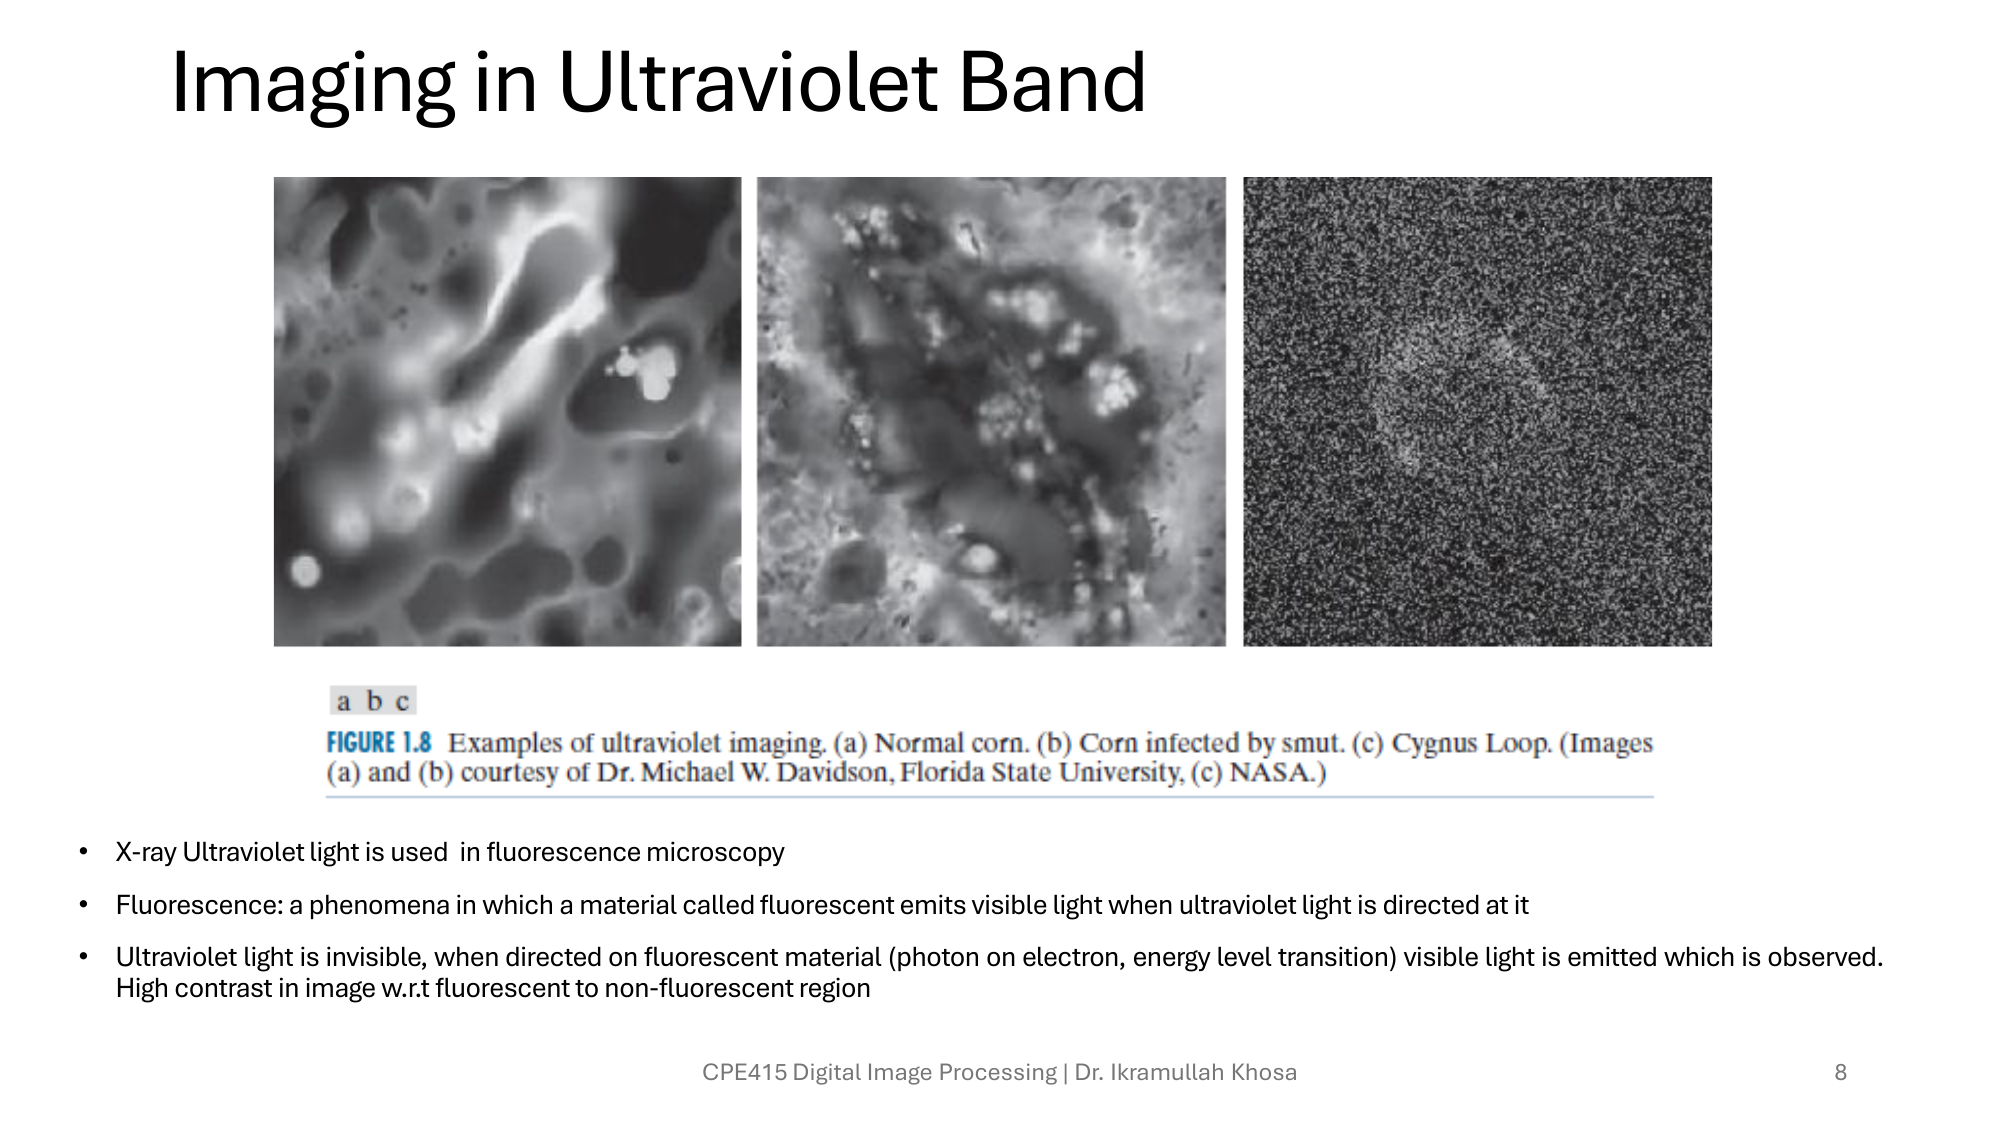
\includegraphics[width=0.9\textwidth]{images/slide1-08.png}
    \caption{Ultraviolet imaging and fluorescence microscopy}
    \label{fig:uv_imaging}
\end{figure}

\begin{deepexplanation}
\textbf{DEEP ANALYSIS - Figure \ref{fig:uv_imaging}: Ultraviolet and Fluorescence Imaging}

\textbf{Fluorescence Microscopy:}

\textbf{The Fluorescence Process:}
\begin{enumerate}
    \item UV light (excitation) hits fluorescent molecule
    \item Electron absorbs photon energy, jumps to excited state
    \item Electron loses some energy to vibrations (heat)
    \item Electron returns to ground state, emitting visible light (longer wavelength than excitation)
\end{enumerate}

\textbf{Stokes Shift:}
\[
\lambda_{emission} > \lambda_{excitation}
\]
The emitted light has lower energy (longer wavelength) than absorbed light.

\textbf{Why Fluorescence Microscopy Is Powerful:}
\begin{itemize}
    \item \textbf{High contrast}: Only fluorescent regions emit light
    \item \textbf{Specificity}: Fluorescent dyes can bind to specific molecules (DNA, proteins, etc.)
    \item \textbf{Dark background}: Non-fluorescent regions appear black
    \item \textbf{Multiple labels}: Different fluorophores with different colors can label different structures
\end{itemize}

\textbf{Applications:}
\begin{itemize}
    \item Cell biology: Visualize specific proteins, organelles
    \item Medical diagnostics: Detect specific biomarkers
    \item Forensics: Detect bodily fluids, fingerprints
    \item Document authentication: Security features
\end{itemize}

\textbf{Technical Note:}
Modern fluorescence microscopy uses filters to:
\begin{itemize}
    \item Excitation filter: Pass only UV/specific wavelength
    \item Dichroic mirror: Reflect excitation, transmit emission
    \item Emission filter: Pass only fluorescence, block excitation
\end{itemize}
\end{deepexplanation}

\subsection{Visible Light Imaging}

\begin{figure}[H]
    \centering
    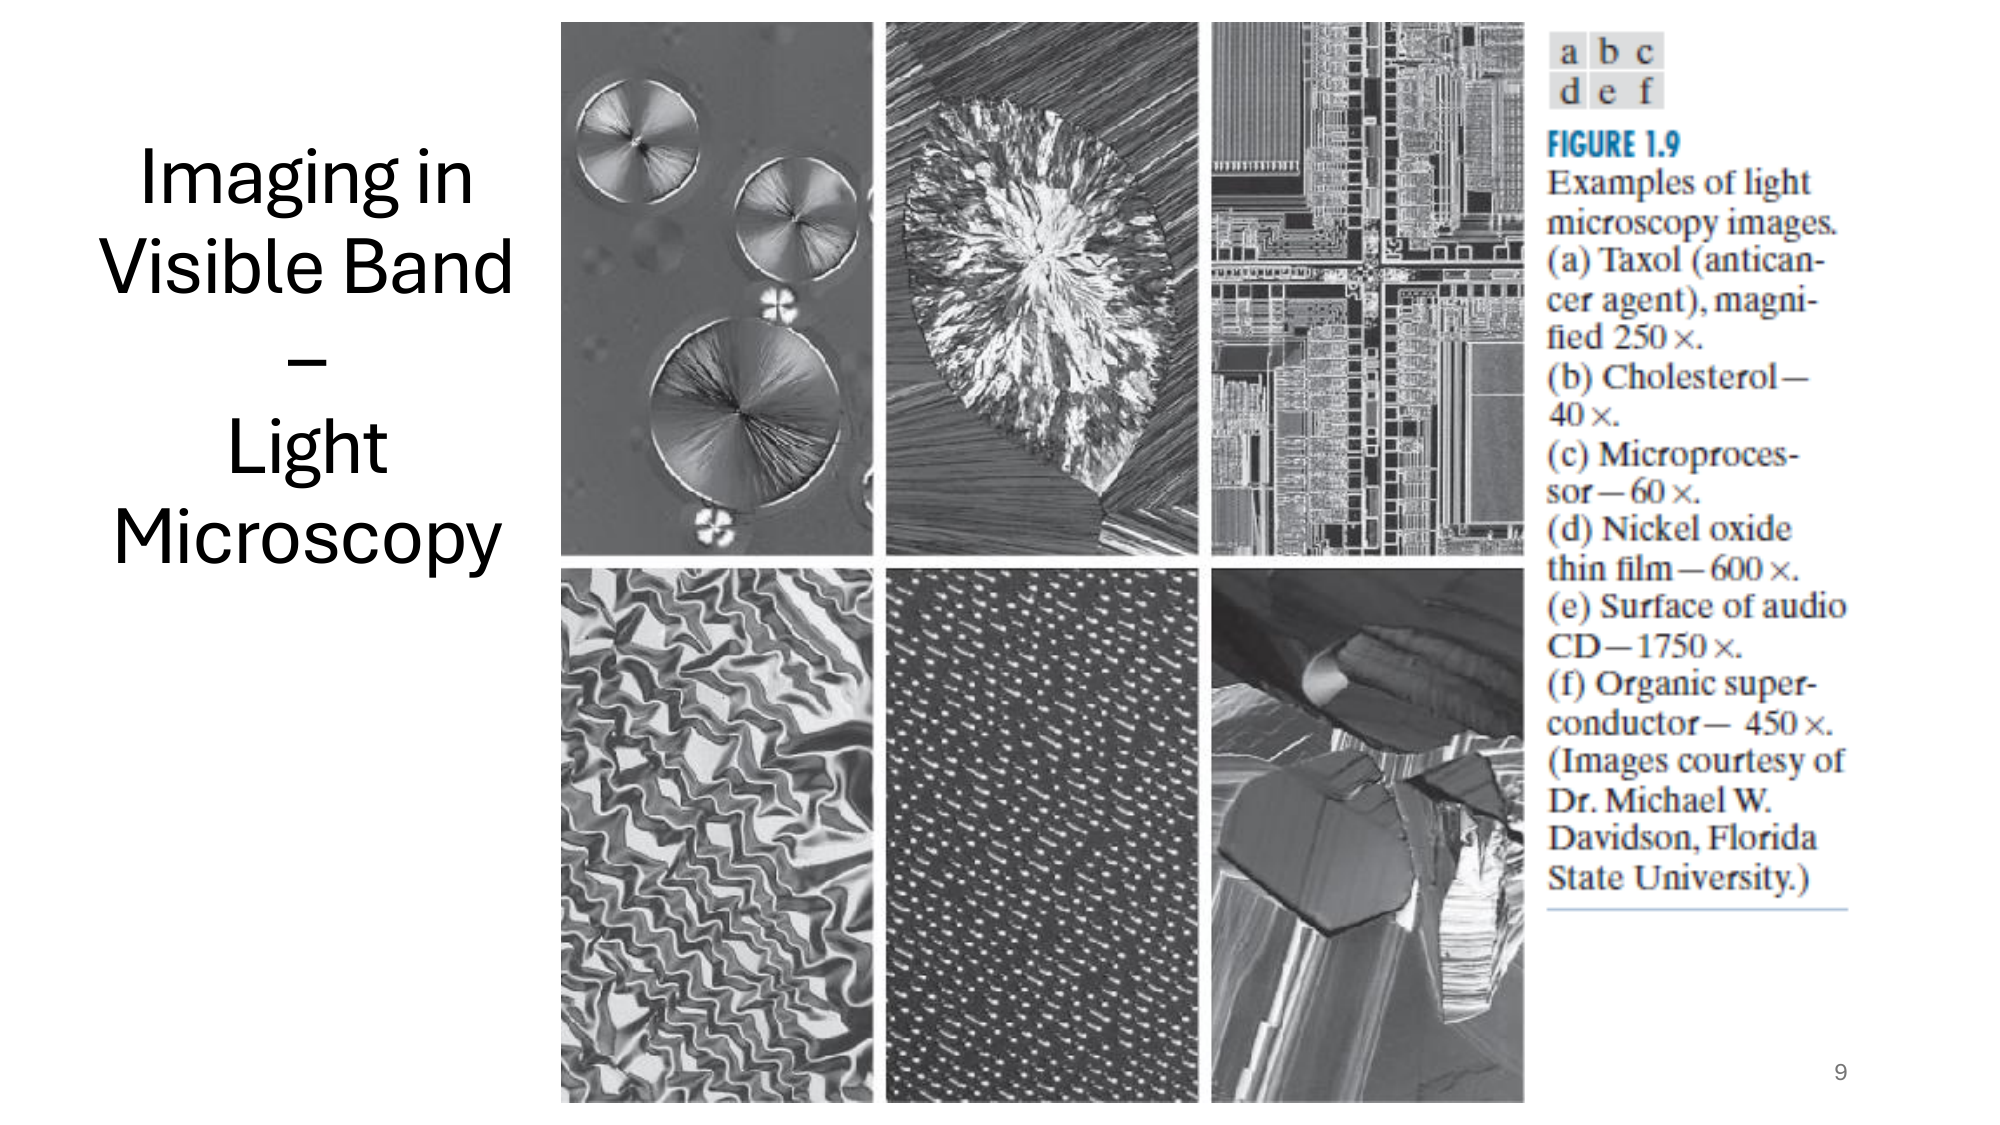
\includegraphics[width=0.9\textwidth]{images/slide1-09.png}
    \caption{Light microscopy in visible band}
    \label{fig:light_microscopy}
\end{figure}

\begin{deepexplanation}
\textbf{DEEP ANALYSIS - Figure \ref{fig:light_microscopy}: Optical Microscopy}

\textbf{Resolution Limit of Light Microscopy:}
The fundamental limit is set by \textbf{diffraction}:
\[
d_{min} = \frac{\lambda}{2 \cdot NA}
\]
where $\lambda$ = wavelength, $NA$ = numerical aperture of lens.

For visible light ($\lambda \approx 500$ nm) and high NA ($\approx 1.4$ with oil immersion):
\[
d_{min} \approx \frac{500}{2 \times 1.4} \approx 180 \text{ nm}
\]

\textbf{This Is Why:}
\begin{itemize}
    \item Light microscopes cannot see individual molecules
    \item Maximum useful magnification $\approx 1000\times$ to $2000\times$
    \item Beyond this, you're just magnifying blur
\end{itemize}

\textbf{Types of Light Microscopy:}
\begin{itemize}
    \item \textbf{Brightfield}: Standard illumination, stained samples
    \item \textbf{Darkfield}: Only scattered light collected, unstained samples
    \item \textbf{Phase contrast}: Converts phase shifts to intensity (unstained living cells)
    \item \textbf{Differential interference contrast (DIC)}: 3D-like appearance
\end{itemize}

\textbf{Image Processing Role:}
\begin{itemize}
    \item Noise reduction
    \item Contrast enhancement
    \item Deconvolution (remove blur)
    \item Cell counting and measurement
    \item 3D reconstruction from focal stacks
\end{itemize}
\end{deepexplanation}

\begin{figure}[H]
    \centering
    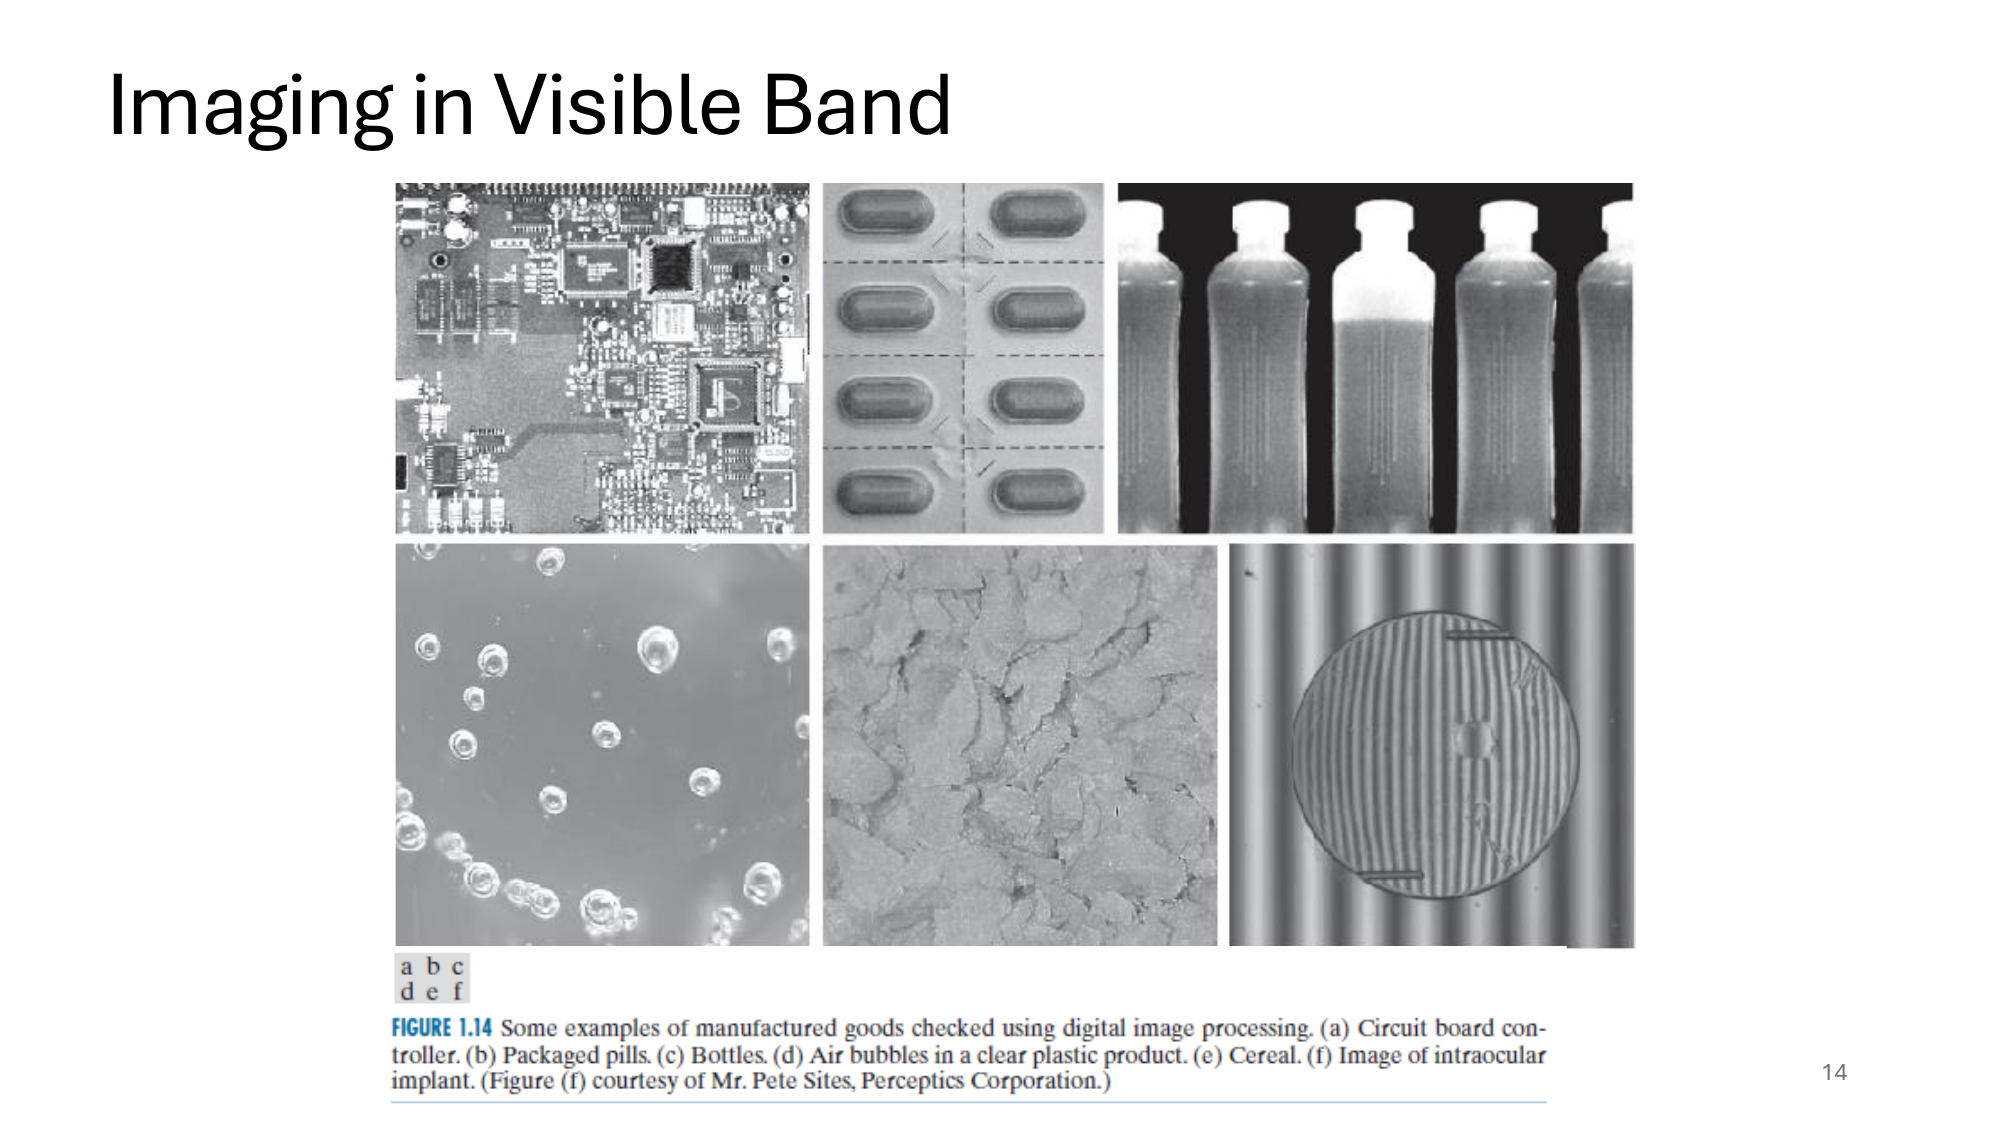
\includegraphics[width=0.9\textwidth]{images/slide1-14.png}
    \caption{Visible light imaging: photography and machine vision}
    \label{fig:visible_imaging}
\end{figure}

\begin{figure}[H]
    \centering
    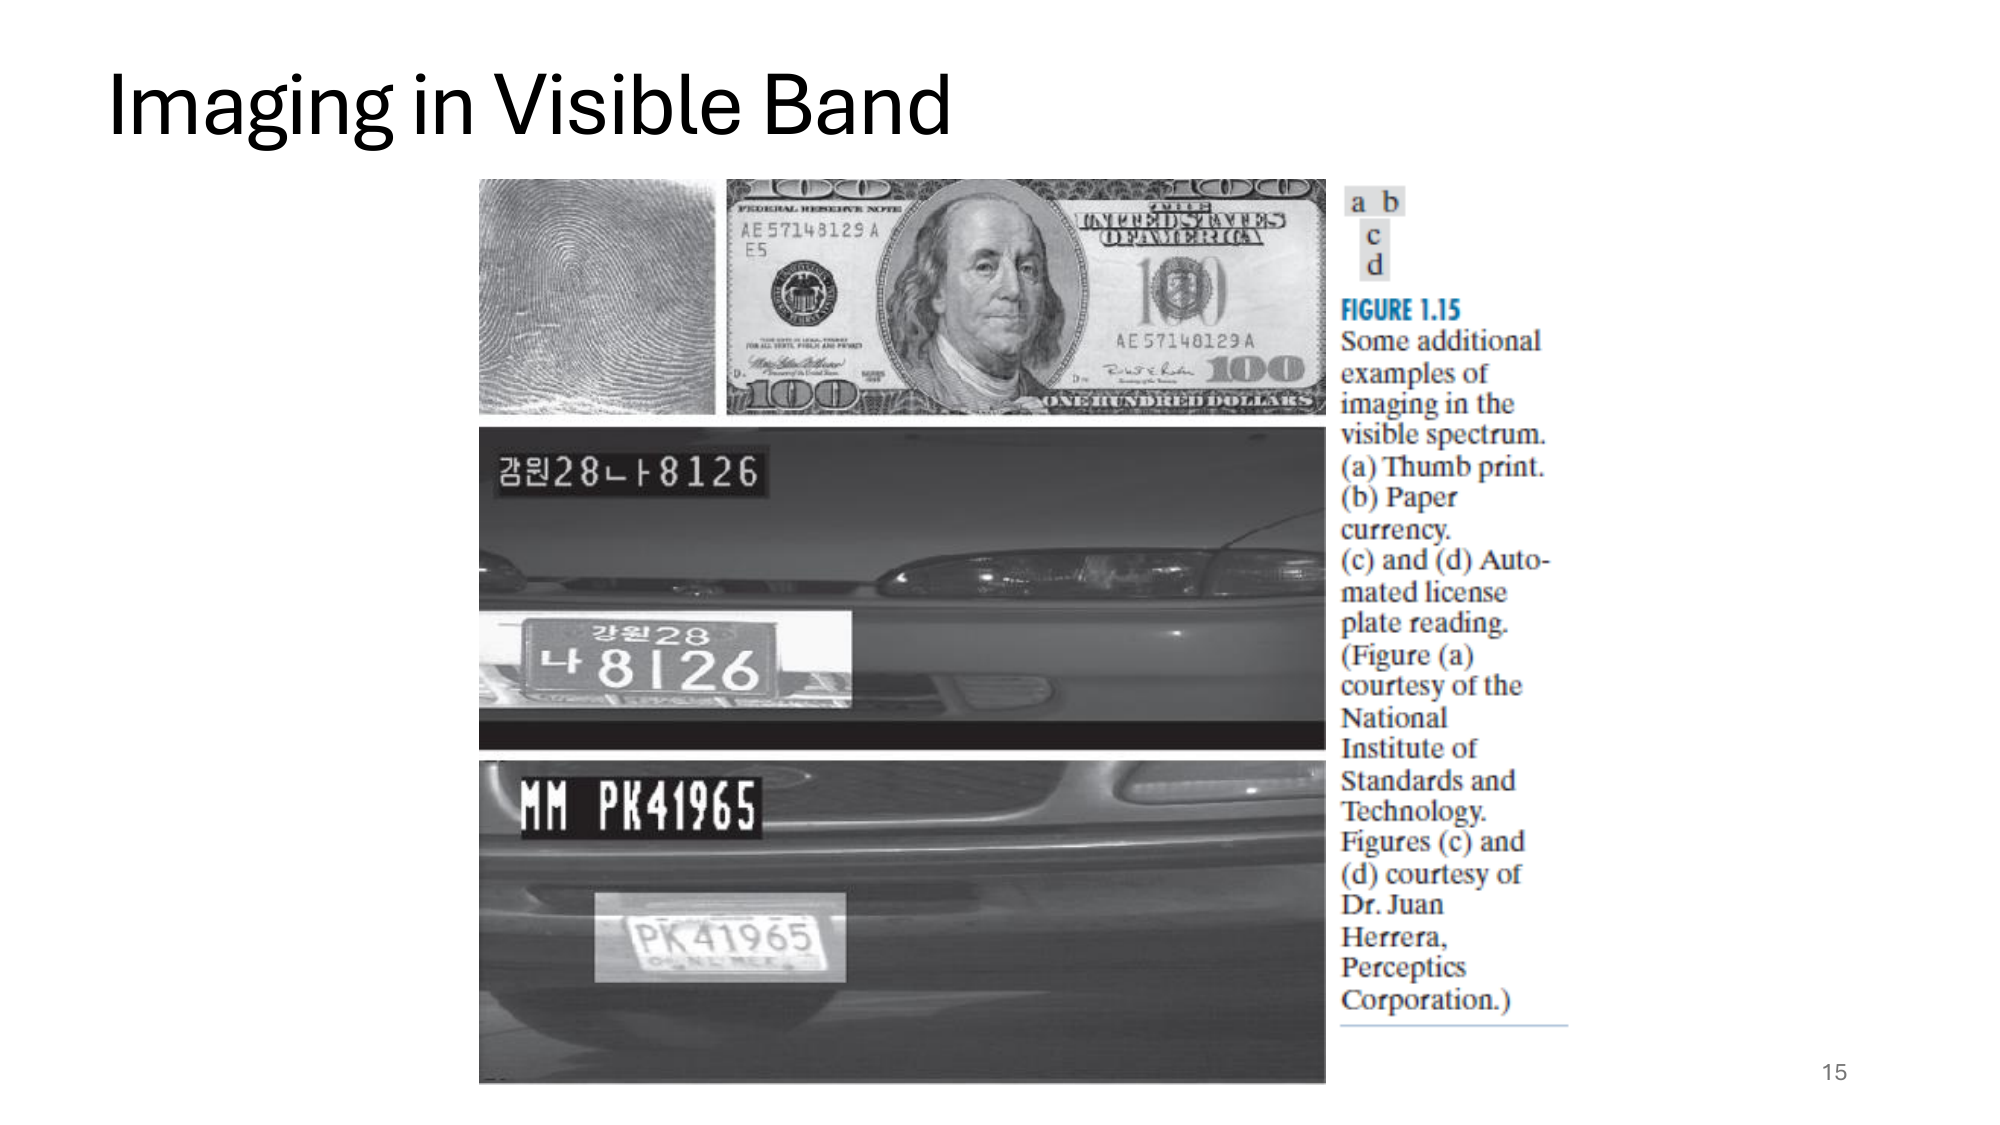
\includegraphics[width=0.9\textwidth]{images/slide1-15.png}
    \caption{More visible light imaging applications}
    \label{fig:visible_apps}
\end{figure}

\begin{deepexplanation}
\textbf{DEEP ANALYSIS - Figures \ref{fig:visible_imaging} and \ref{fig:visible_apps}: Visible Light Applications}

\textbf{Why Visible Light Imaging Is Most Common:}
\begin{itemize}
    \item Matches human vision (intuitive interpretation)
    \item Abundant natural illumination (sunlight)
    \item Inexpensive sensors and optics
    \item Color provides rich information
\end{itemize}

\textbf{Key Applications:}

\textbf{1. Consumer Photography:}
\begin{itemize}
    \item Smartphones now have sophisticated image processing
    \item HDR, portrait mode, night mode all use DIP algorithms
\end{itemize}

\textbf{2. Industrial Machine Vision:}
\begin{itemize}
    \item Quality inspection: Detect defects in manufactured parts
    \item Guidance: Robots use vision for positioning
    \item OCR: Read text on labels, packaging
    \item Measurement: Precise dimensional verification
\end{itemize}

\textbf{3. Surveillance and Security:}
\begin{itemize}
    \item Face recognition
    \item Motion detection
    \item License plate recognition
    \item Crowd monitoring
\end{itemize}

\textbf{4. Medical Imaging:}
\begin{itemize}
    \item Dermatology: Skin lesion analysis
    \item Ophthalmology: Retinal imaging
    \item Endoscopy: Internal body visualization
    \item Pathology: Tissue slide analysis
\end{itemize}
\end{deepexplanation}

\subsection{Infrared Imaging}

\begin{figure}[H]
    \centering
    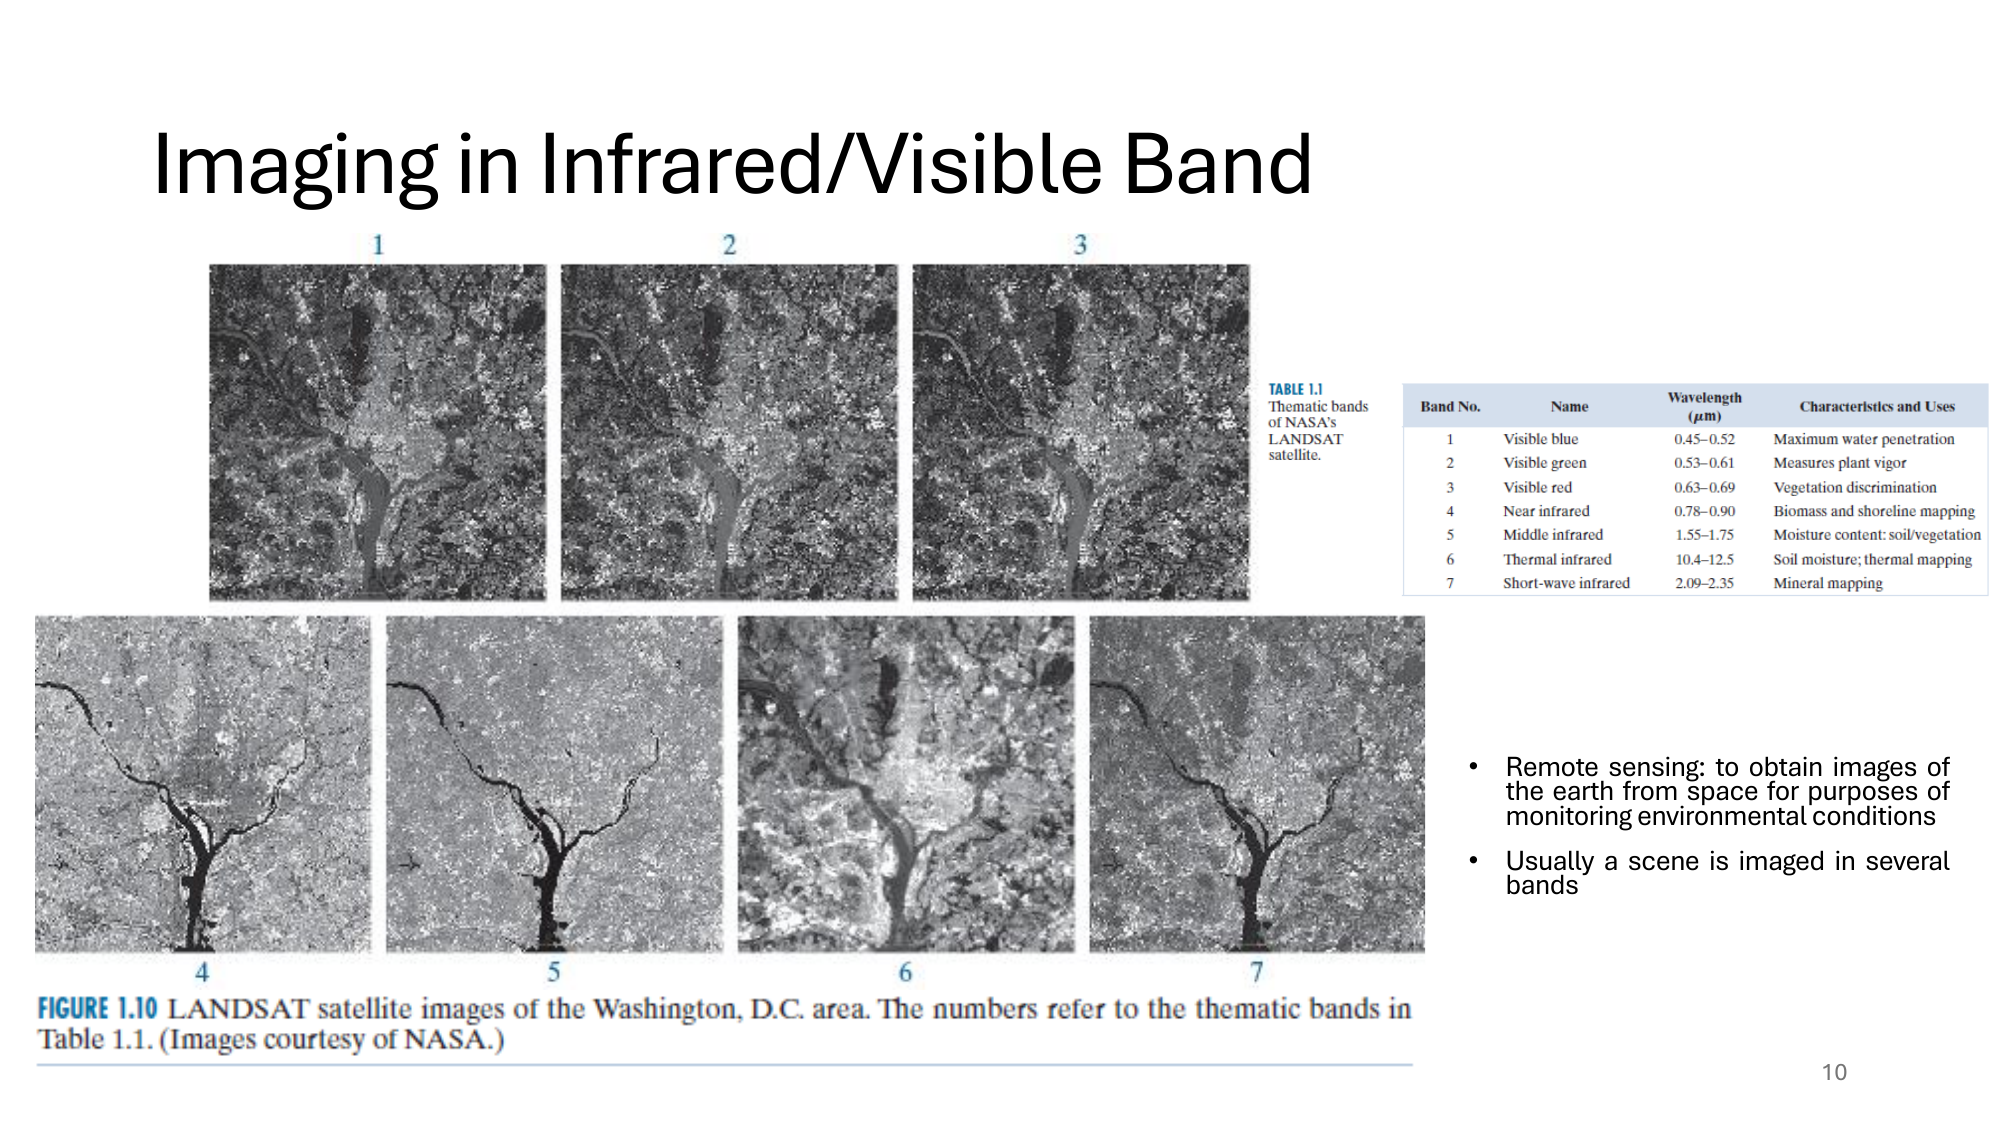
\includegraphics[width=0.9\textwidth]{images/slide1-10.png}
    \caption{Infrared and visible band combined imaging for remote sensing}
    \label{fig:ir_remote}
\end{figure}

\begin{deepexplanation}
\textbf{DEEP ANALYSIS - Figure \ref{fig:ir_remote}: Multispectral Remote Sensing}

\textbf{What Infrared Reveals That Visible Doesn't:}

\textbf{Near Infrared (NIR, 700 nm -- 1.4 µm):}
\begin{itemize}
    \item \textbf{Vegetation health}: Healthy plants strongly reflect NIR
    \item Chlorophyll absorbs red but reflects NIR
    \item NDVI (Normalized Difference Vegetation Index):
    \[
    NDVI = \frac{NIR - Red}{NIR + Red}
    \]
    \item $NDVI \approx 0.8$: Healthy vegetation; $NDVI \approx 0$: No vegetation
\end{itemize}

\textbf{Remote Sensing:}
\begin{itemize}
    \item Satellites capture multiple spectral bands simultaneously
    \item Combine bands for ``false color'' images revealing hidden information
    \item Common band combinations:
    \begin{itemize}
        \item Natural color: RGB = Red, Green, Blue
        \item Color infrared: RGB = NIR, Red, Green (vegetation appears red)
        \item Agriculture: RGB = SWIR, NIR, Blue (crop health)
    \end{itemize}
\end{itemize}

\textbf{Why Multispectral Imaging Works:}
Different materials have different \textbf{spectral signatures} --- how they reflect/absorb at each wavelength. By capturing multiple bands, we can distinguish materials that look identical in visible light.
\end{deepexplanation}

\begin{figure}[H]
    \centering
    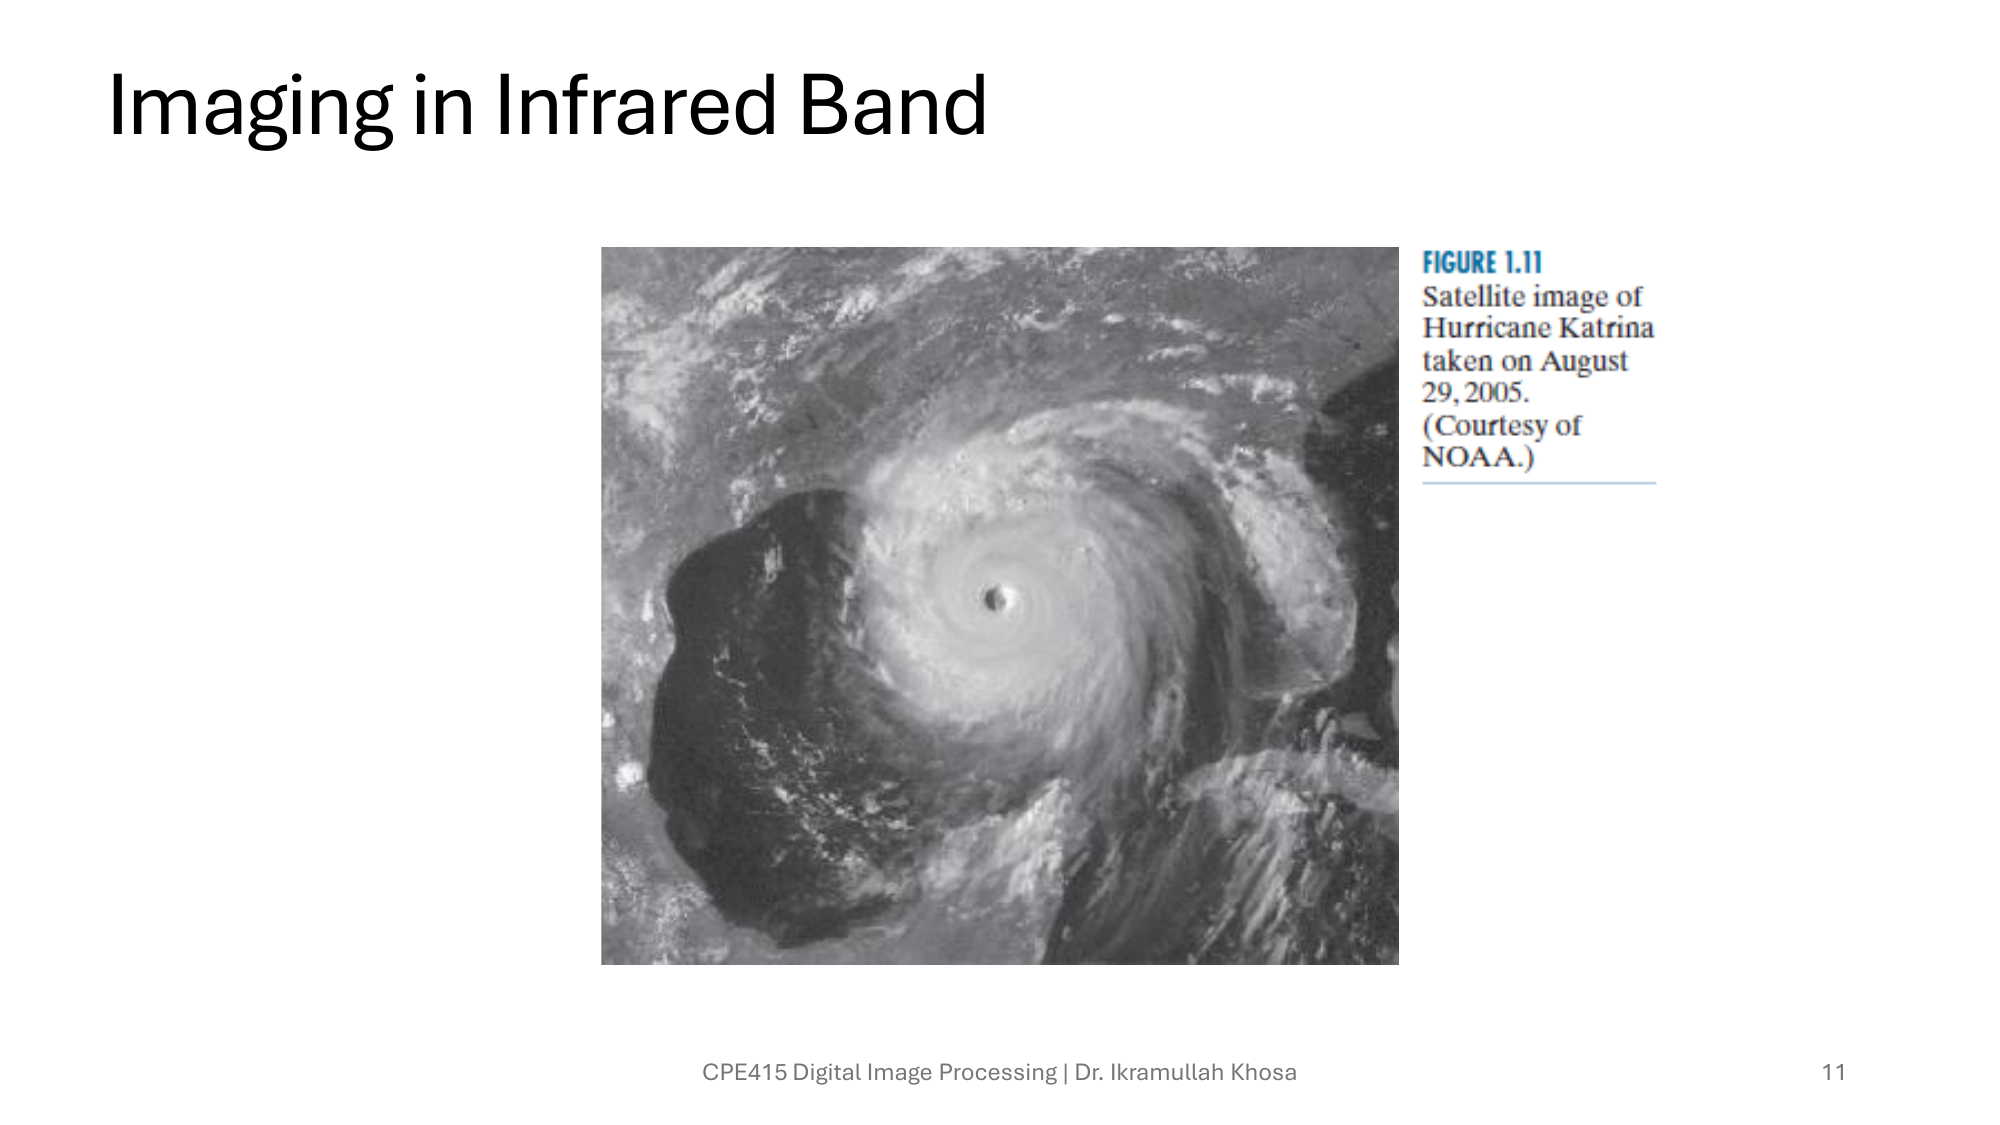
\includegraphics[width=0.9\textwidth]{images/slide1-11.png}
    \caption{Thermal infrared imaging}
    \label{fig:thermal}
\end{figure}

\begin{deepexplanation}
\textbf{DEEP ANALYSIS - Figure \ref{fig:thermal}: Thermal Imaging}

\textbf{The Physics of Thermal Imaging:}
All objects above absolute zero emit thermal radiation. The peak wavelength depends on temperature:

\textbf{Wien's Displacement Law:}
\[
\lambda_{peak} = \frac{2898 \text{ µm·K}}{T}
\]

\textbf{Examples:}
\begin{itemize}
    \item Human body (310 K): $\lambda_{peak} \approx 9.4$ µm (mid-IR)
    \item Room temperature (293 K): $\lambda_{peak} \approx 9.9$ µm
    \item Hot machinery (400 K): $\lambda_{peak} \approx 7.2$ µm
\end{itemize}

\textbf{Key Feature:}
Thermal imaging requires \textbf{no external illumination} --- objects are their own light source!

\textbf{Applications:}
\begin{itemize}
    \item \textbf{Night vision}: See in complete darkness
    \item \textbf{Building inspection}: Detect heat leaks, insulation failures
    \item \textbf{Electrical inspection}: Find overheating components
    \item \textbf{Medical}: Detect inflammation, circulation problems
    \item \textbf{Search and rescue}: Find people in smoke/darkness
    \item \textbf{Military}: Target detection regardless of lighting
\end{itemize}

\textbf{Technical Challenges:}
\begin{itemize}
    \item IR sensors more expensive than visible sensors
    \item Atmospheric absorption in certain bands
    \item Lower resolution than visible cameras
    \item Must be cooled for highest sensitivity (LWIR)
\end{itemize}
\end{deepexplanation}

\begin{figure}[H]
    \centering
    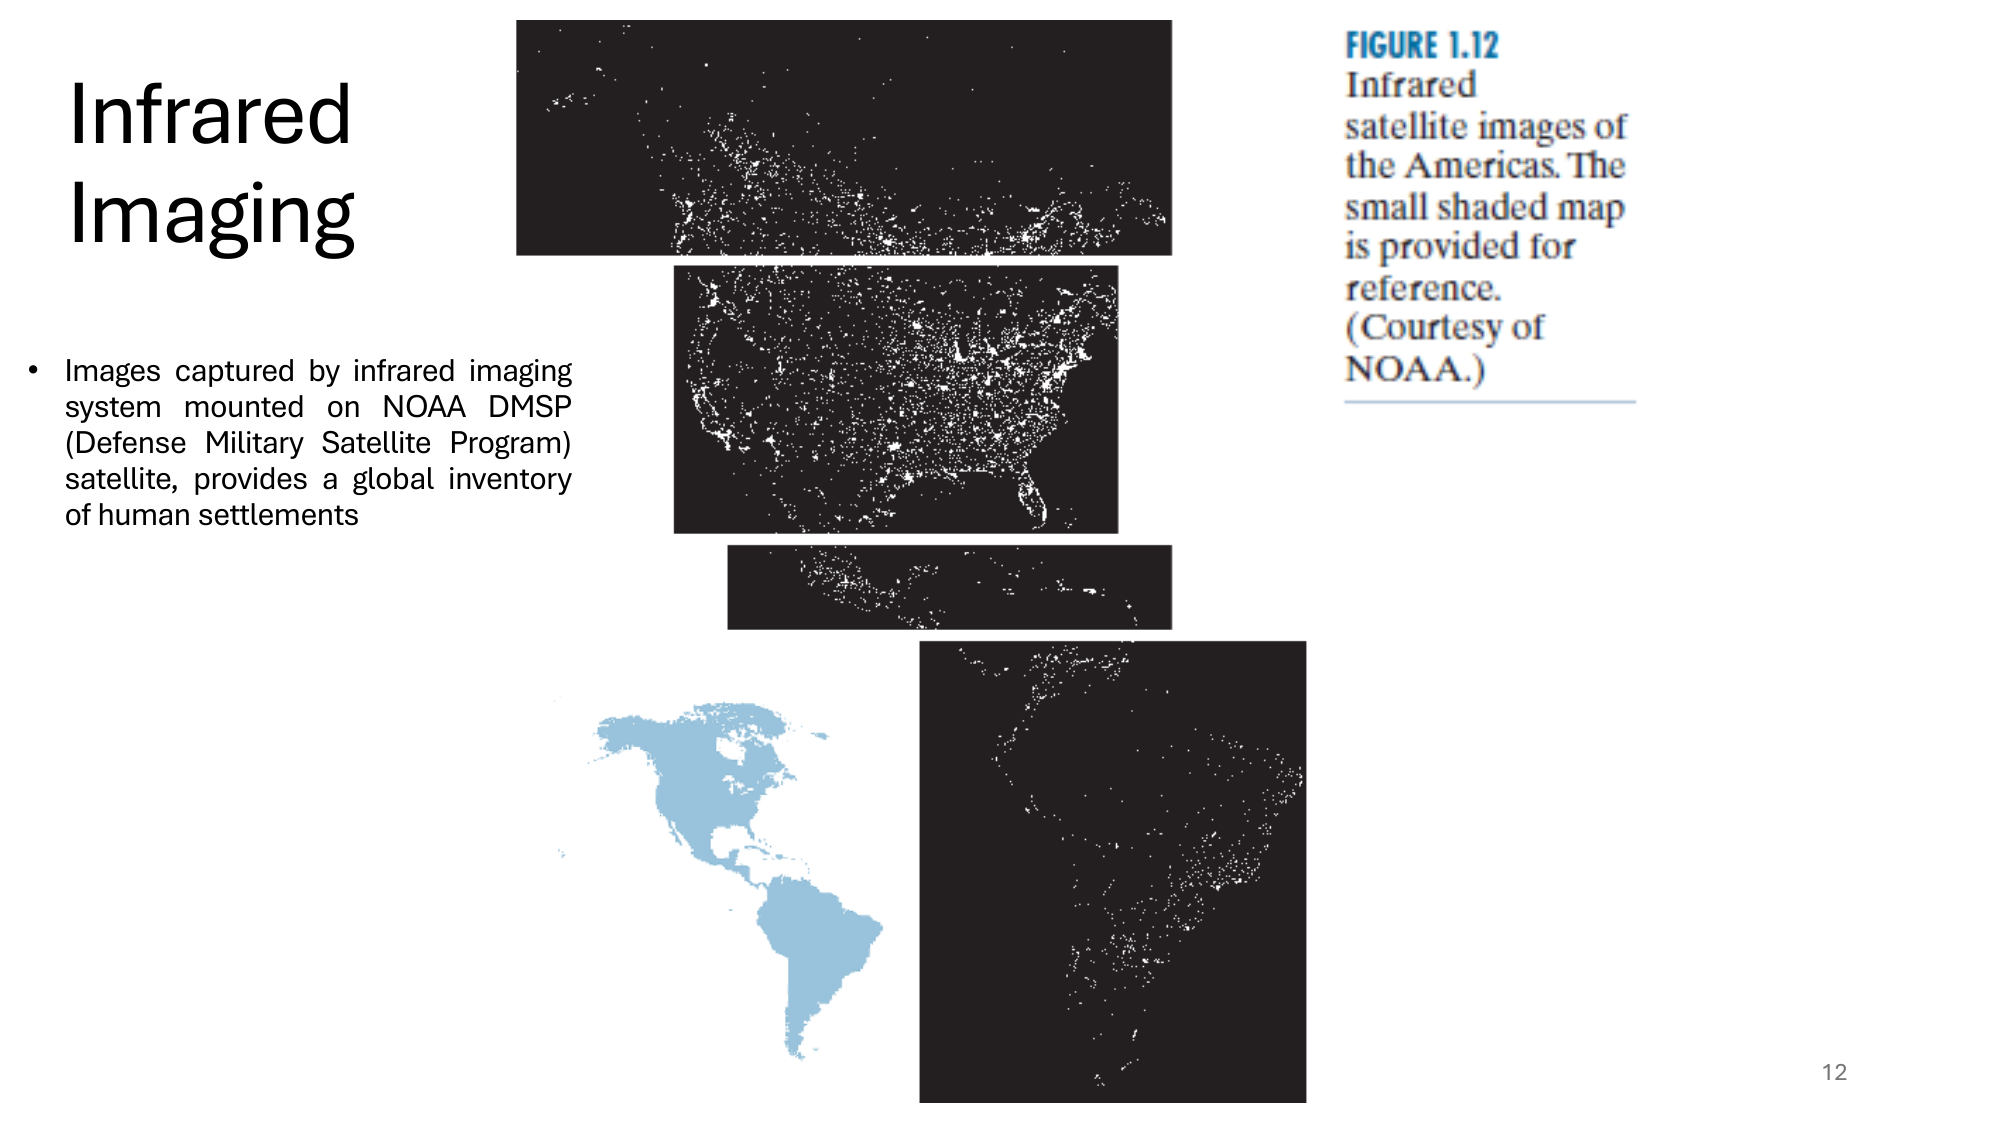
\includegraphics[width=0.9\textwidth]{images/slide1-12.png}
    \caption{Satellite infrared imaging of human settlements}
    \label{fig:satellite_ir}
\end{figure}

\begin{deepexplanation}
\textbf{DEEP ANALYSIS - Figure \ref{fig:satellite_ir}: Global Night-Time Light Mapping}

\textbf{What Satellite IR/Night-Light Imaging Reveals:}

\textbf{DMSP (Defense Meteorological Satellite Program):}
\begin{itemize}
    \item Captures visible and infrared images of Earth at night
    \item City lights visible from space
    \item Provides global inventory of human settlements
\end{itemize}

\textbf{What the Data Shows:}
\begin{itemize}
    \item Population distribution (more lights = more people)
    \item Economic development (more lights = more activity)
    \item Energy consumption patterns
    \item Urbanization over time (comparing years)
\end{itemize}

\textbf{Scientific Applications:}
\begin{itemize}
    \item GDP estimation from light intensity
    \item Poverty mapping
    \item Light pollution studies
    \item Disaster response (power outage detection)
    \item Conflict monitoring (changes in lighting patterns)
\end{itemize}

\textbf{Image Processing Challenges:}
\begin{itemize}
    \item Clouds obscure surface
    \item Fires can be confused with lights
    \item Aurora affects polar regions
    \item Moonlight reflection
    \item Sensor saturation in bright cities
\end{itemize}
\end{deepexplanation}

\begin{figure}[H]
    \centering
    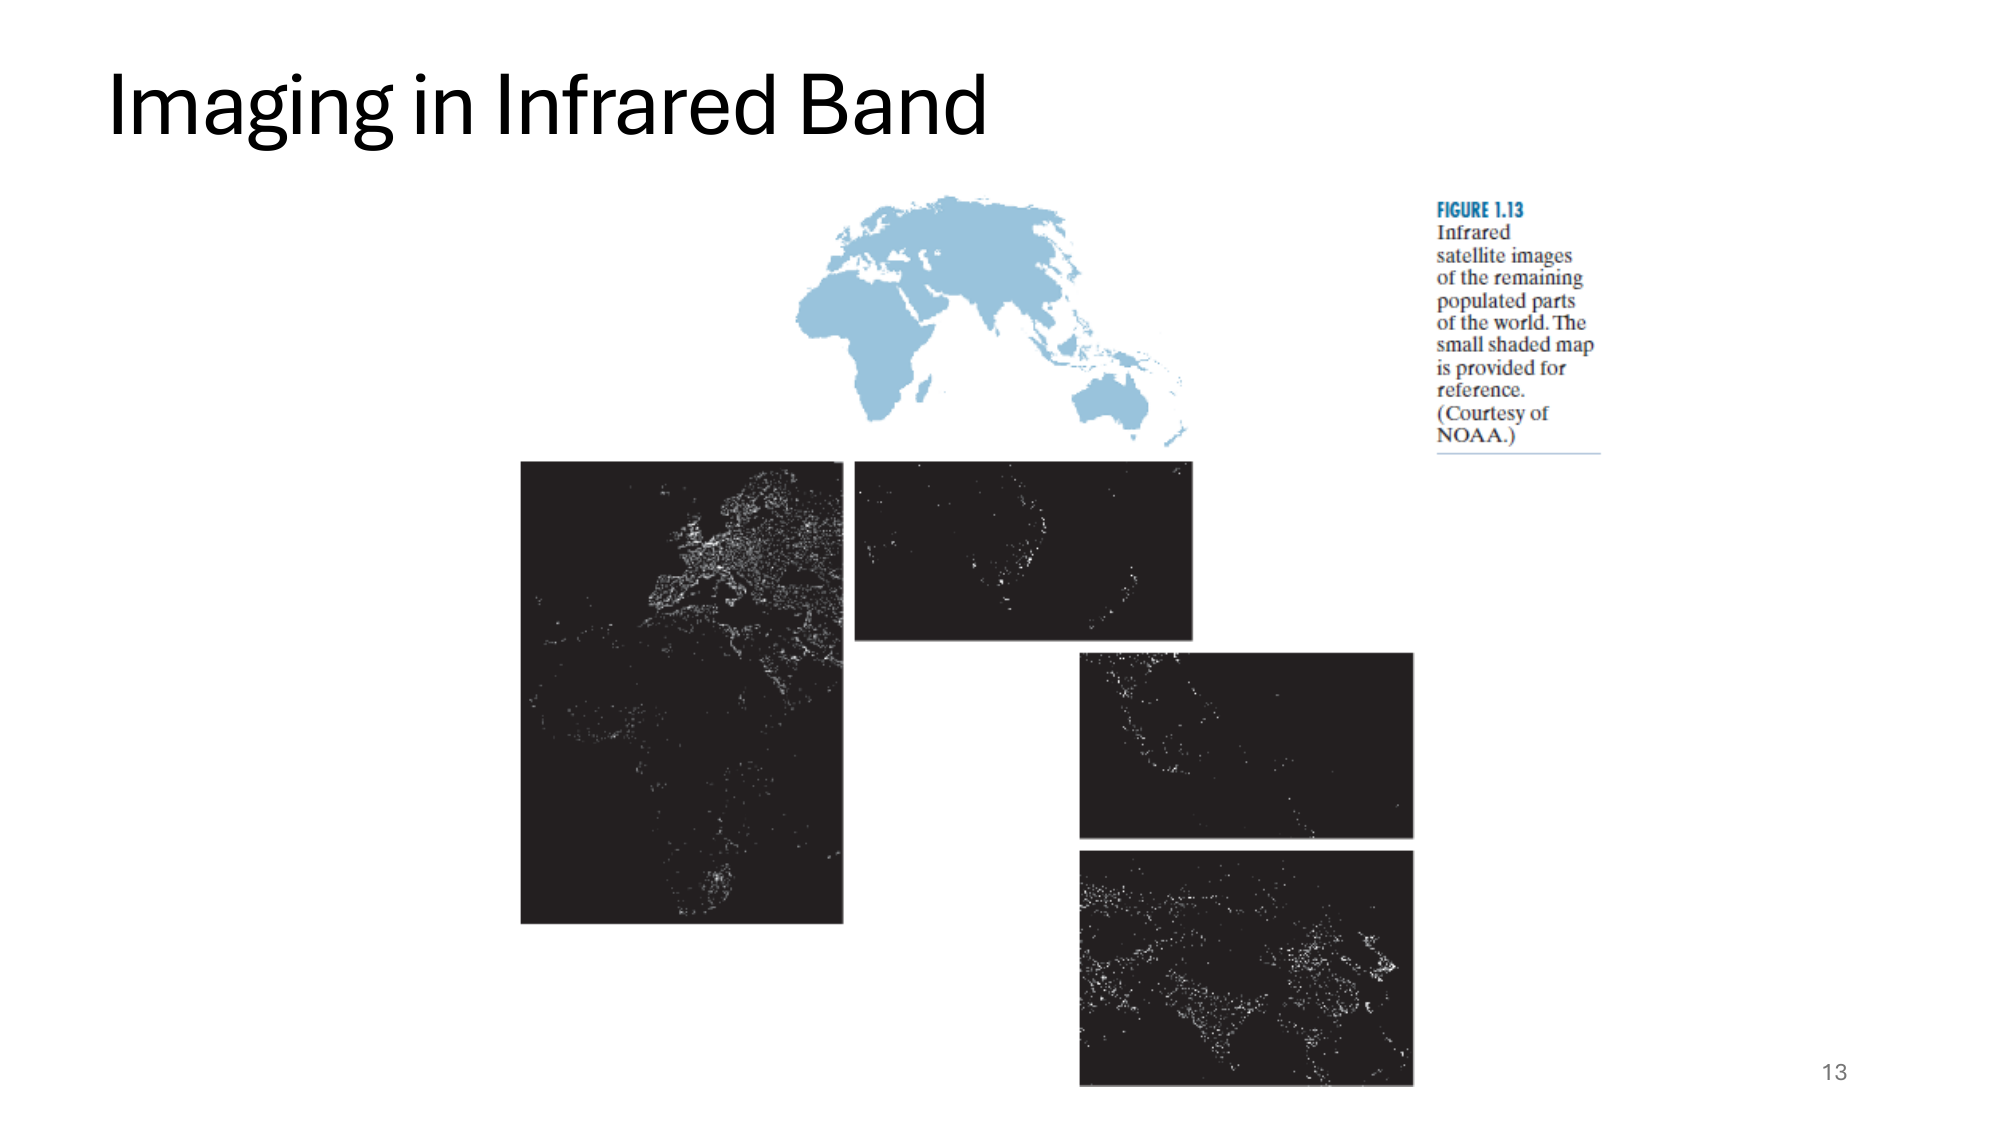
\includegraphics[width=0.9\textwidth]{images/slide1-13.png}
    \caption{Infrared imaging applications}
    \label{fig:ir_apps}
\end{figure}


\subsection{Microwave Imaging}

\begin{figure}[H]
    \centering
    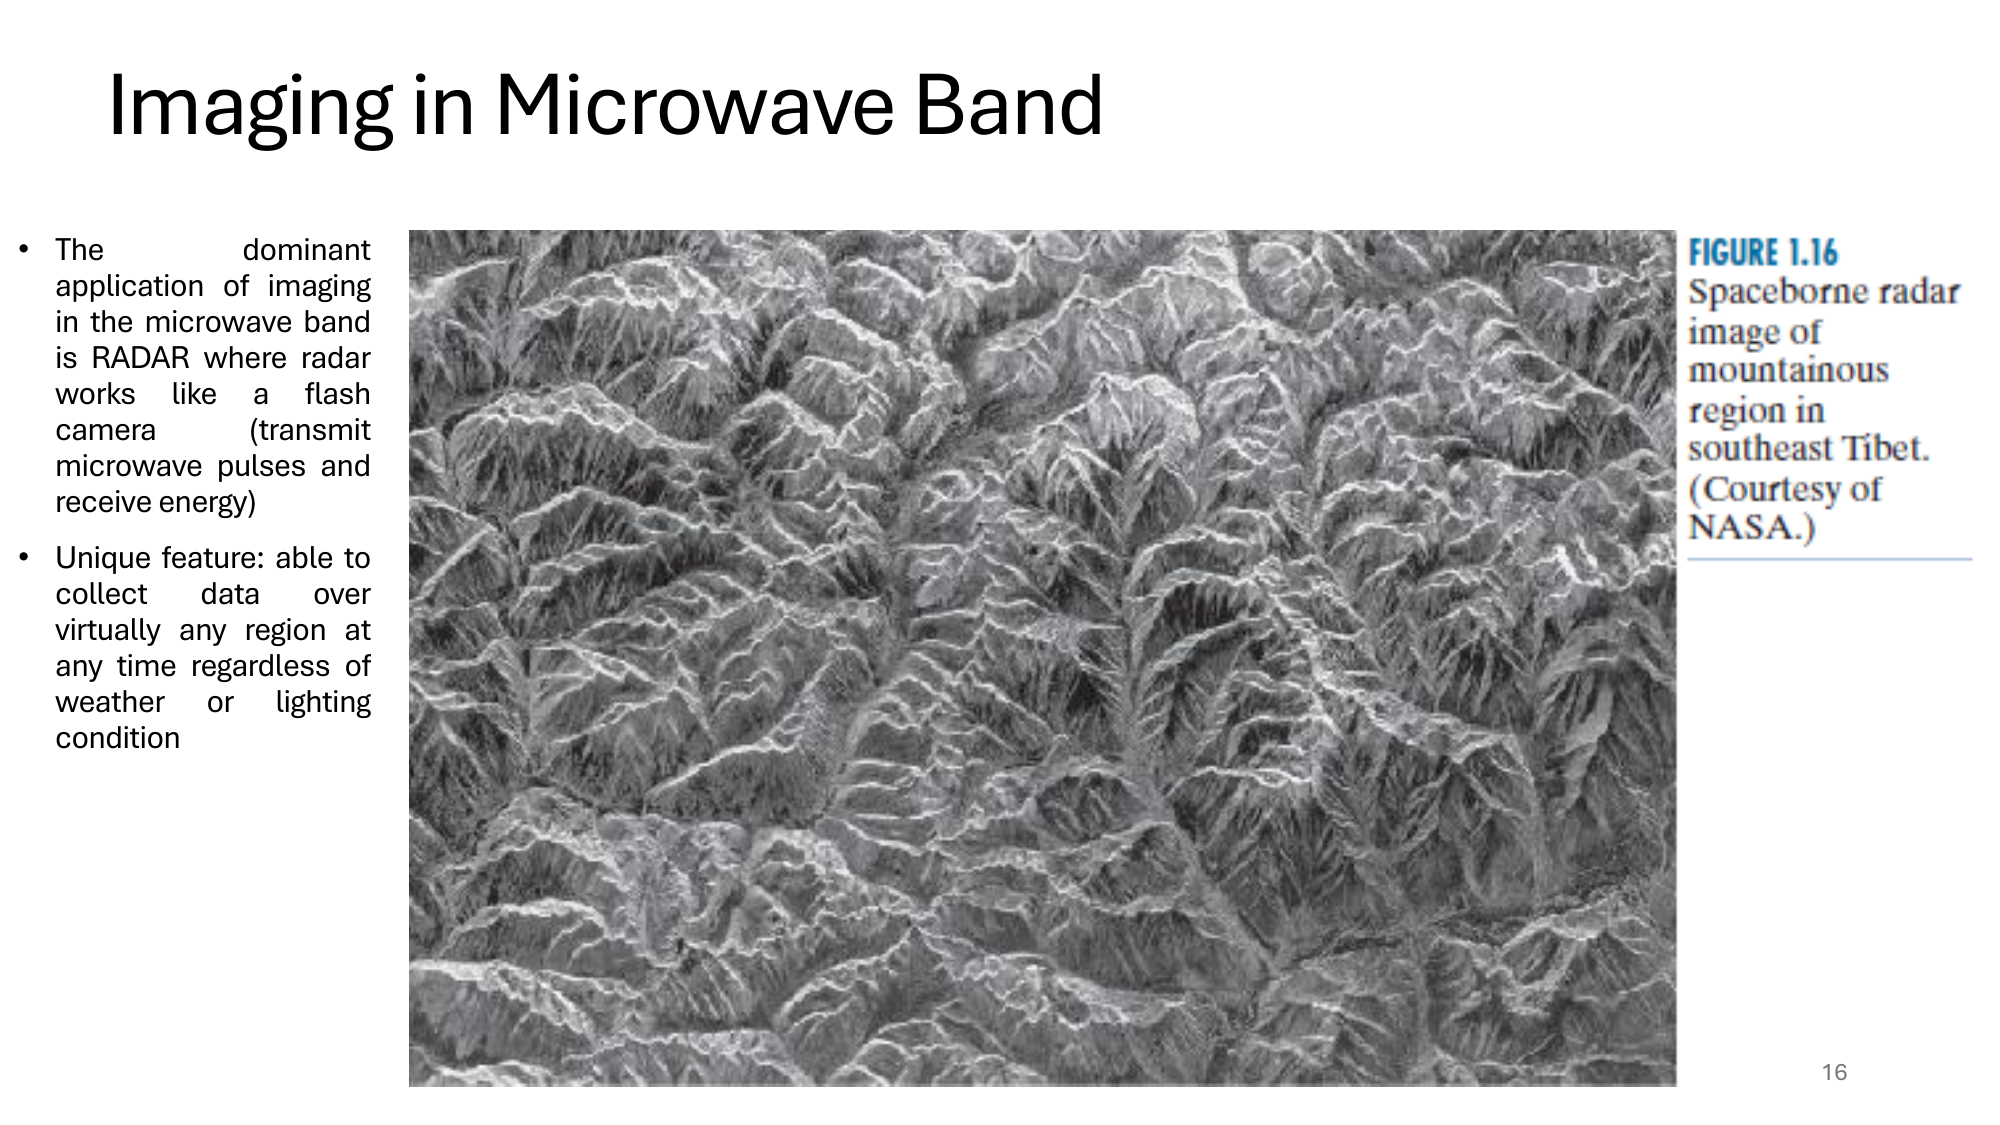
\includegraphics[width=0.9\textwidth]{images/slide1-16.png}
    \caption{Microwave imaging: RADAR and SAR}
    \label{fig:microwave}
\end{figure}

\begin{deepexplanation}
\textbf{DEEP ANALYSIS - Figure \ref{fig:microwave}: Radar Imaging}

\textbf{How RADAR Imaging Works:}
RADAR = Radio Detection And Ranging

\textbf{The Principle:}
\begin{enumerate}
    \item Transmit microwave pulse toward scene
    \item Pulse reflects off objects
    \item Receive echoes at antenna
    \item Time delay gives distance: $R = \frac{c \cdot t}{2}$
    \item Echo strength gives information about surface properties
\end{enumerate}

\textbf{Synthetic Aperture Radar (SAR):}
\begin{itemize}
    \item Problem: Resolution $\propto$ antenna size; can't fit large antenna on aircraft/satellite
    \item Solution: Use \textbf{motion} of platform to synthesize a large antenna
    \item As platform moves, it collects data from many positions
    \item Coherent processing combines these into one high-resolution image
    \item Effective aperture length = distance traveled during imaging
\end{itemize}

\textbf{SAR Resolution:}
\begin{itemize}
    \item Range resolution: $\Delta R = \frac{c}{2B}$ where $B$ = bandwidth
    \item Azimuth resolution: $\Delta_{az} = \frac{D}{2}$ where $D$ = real antenna length
    \item Independent of distance (unlike optical systems)!
\end{itemize}

\textbf{Unique Advantages:}
\begin{itemize}
    \item \textbf{All-weather}: Microwaves penetrate clouds, rain, fog
    \item \textbf{Day/night}: Active system, doesn't need sunlight
    \item \textbf{Penetration}: Can see through vegetation, dry sand
    \item \textbf{Surface texture}: Rough vs smooth surfaces reflect differently
\end{itemize}

\textbf{Applications:}
\begin{itemize}
    \item Terrain mapping
    \item Ship and aircraft detection
    \item Ocean monitoring (waves, currents, oil spills)
    \item Deforestation monitoring
    \item Archaeology (finding buried structures)
\end{itemize}
\end{deepexplanation}

\subsection{Radio Wave Imaging (MRI)}

\begin{figure}[H]
    \centering
    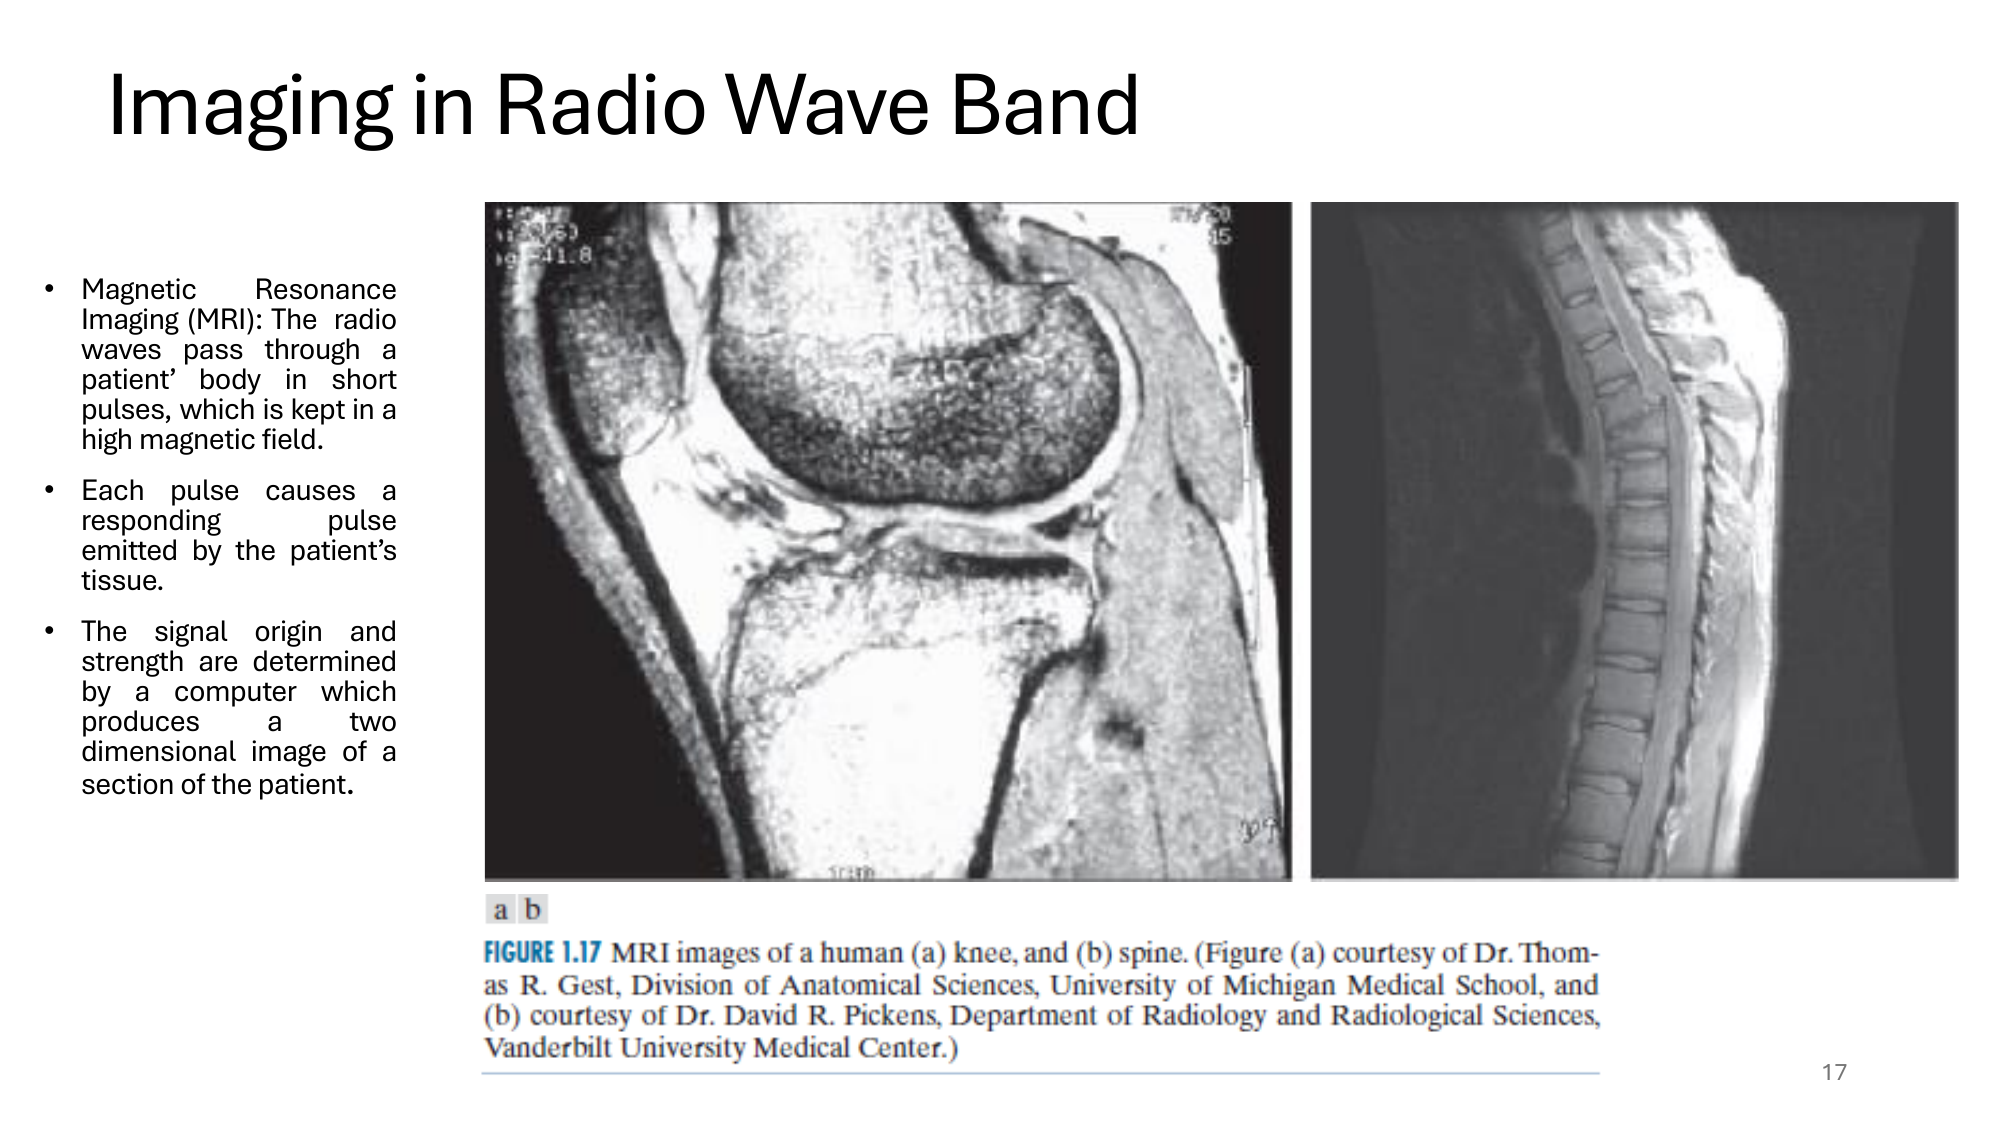
\includegraphics[width=0.9\textwidth]{images/slide1-17.png}
    \caption{Magnetic Resonance Imaging (MRI) using radio waves}
    \label{fig:mri}
\end{figure}

\begin{deepexplanation}
\textbf{DEEP ANALYSIS - Figure \ref{fig:mri}: MRI Physics and Imaging}

\textbf{The Physics of MRI:}

\textbf{1. Nuclear Spin:}
\begin{itemize}
    \item Protons (hydrogen nuclei) have intrinsic spin (quantum property)
    \item Spin creates a tiny magnetic moment (like a bar magnet)
    \item Normally, spins are randomly oriented $\rightarrow$ no net magnetization
\end{itemize}

\textbf{2. External Magnetic Field ($B_0$):}
\begin{itemize}
    \item Place patient in strong magnetic field (1.5--7 Tesla typical)
    \item Spins align with field (parallel or anti-parallel)
    \item Slight excess parallel $\rightarrow$ net magnetization along field
\end{itemize}

\textbf{3. RF Pulse Excitation:}
\begin{itemize}
    \item Apply radio frequency pulse at the \textbf{Larmor frequency}:
    \[
    f_L = \gamma \cdot B_0
    \]
    where $\gamma = 42.58$ MHz/T for hydrogen
    \item For 1.5T: $f_L \approx 64$ MHz (radio frequency!)
    \item RF pulse tips magnetization away from equilibrium
\end{itemize}

\textbf{4. Relaxation and Signal:}
\begin{itemize}
    \item After RF pulse, magnetization returns to equilibrium
    \item As it does, it induces a signal in receiver coil
    \item Two relaxation time constants: $T_1$ (spin-lattice) and $T_2$ (spin-spin)
    \item Different tissues have different $T_1$, $T_2$ $\rightarrow$ \textbf{contrast}!
\end{itemize}

\textbf{5. Spatial Encoding:}
\begin{itemize}
    \item Add gradient magnetic fields that vary spatially
    \item Larmor frequency now depends on position
    \item Frequency encodes location (Fourier transform to get image)
\end{itemize}

\textbf{Why MRI Is Powerful:}
\begin{itemize}
    \item \textbf{No ionizing radiation} (safe for repeated use)
    \item \textbf{Excellent soft tissue contrast} (unlike CT)
    \item \textbf{Arbitrary plane imaging} (axial, sagittal, coronal, oblique)
    \item \textbf{Functional imaging possible} (fMRI for brain activity)
\end{itemize}
\end{deepexplanation}

\subsection{Multi-Spectral Imaging Example}

\begin{figure}[H]
    \centering
    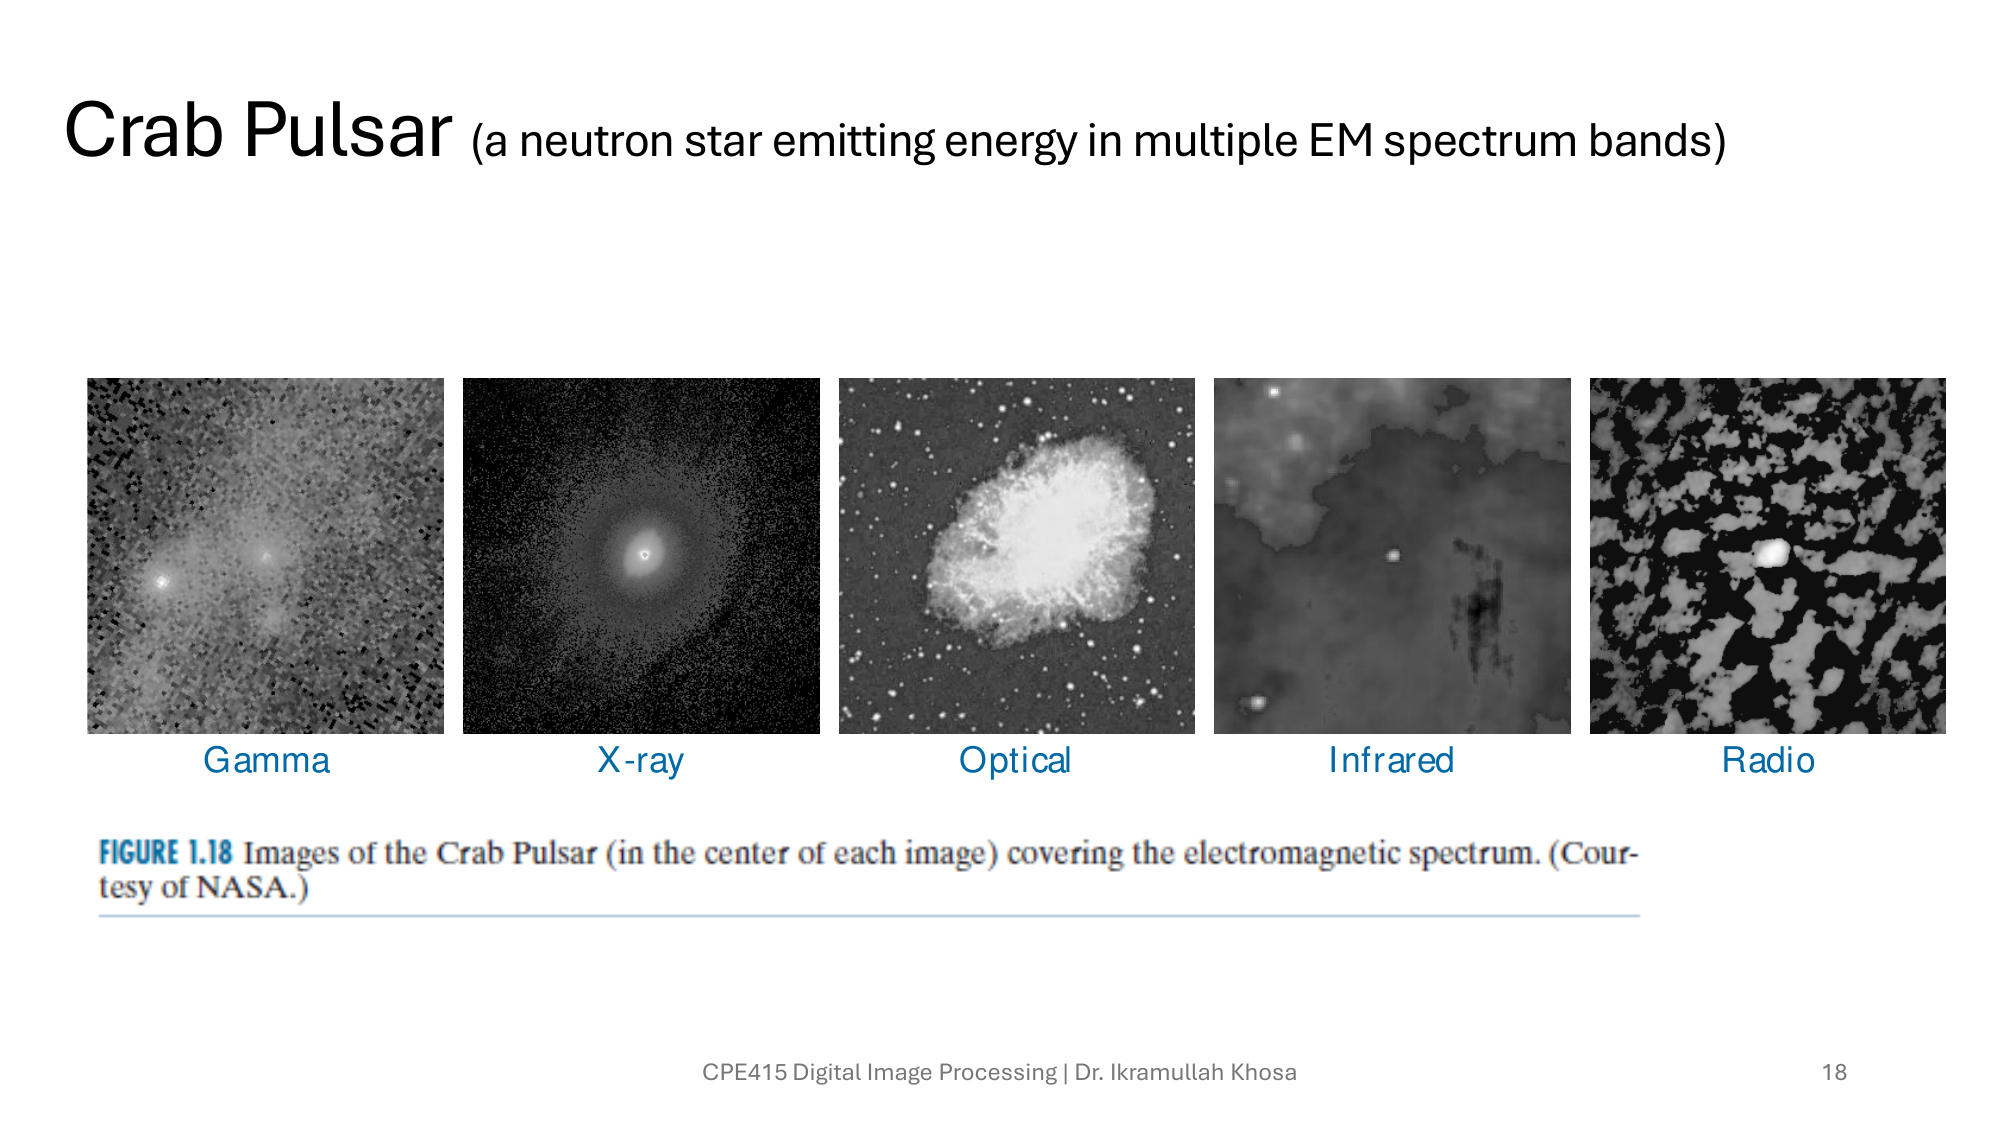
\includegraphics[width=0.95\textwidth]{images/slide1-18.png}
    \caption{Crab Pulsar imaged across multiple EM bands}
    \label{fig:crab_pulsar}
\end{figure}

\begin{deepexplanation}
\textbf{DEEP ANALYSIS - Figure \ref{fig:crab_pulsar}: Multi-Wavelength Astronomy}

\textbf{The Crab Nebula and Pulsar:}
\begin{itemize}
    \item Remnant of a supernova explosion observed in 1054 AD
    \item At center: A \textbf{pulsar} (rapidly rotating neutron star)
    \item The pulsar spins 30 times per second, emitting radiation across entire EM spectrum
\end{itemize}

\textbf{What Each Wavelength Reveals:}

\textbf{Gamma Rays:}
\begin{itemize}
    \item Highest-energy processes
    \item Particle acceleration near pulsar
    \item Compact, bright source at pulsar location
\end{itemize}

\textbf{X-Rays:}
\begin{itemize}
    \item Hot gas ($> 10^6$ K)
    \item Shows jets from pulsar
    \item Ring structures from pulsar wind
\end{itemize}

\textbf{Optical (Visible):}
\begin{itemize}
    \item The familiar ``crab'' shape of the nebula
    \item Filaments of gas excited by pulsar radiation
    \item Synchrotron radiation from electrons
\end{itemize}

\textbf{Infrared:}
\begin{itemize}
    \item Dust mixed with gas
    \item Cooler material in outer regions
    \item Extends further than visible image
\end{itemize}

\textbf{Radio:}
\begin{itemize}
    \item Synchrotron radiation (electrons spiraling in magnetic field)
    \item Largest extent of any band
    \item Pulsations at 30 Hz
\end{itemize}

\textbf{The Power of Multi-Spectral Analysis:}
Each band reveals different physical processes. Combined, they give a complete picture of this complex object that no single band could provide.
\end{deepexplanation}

%==============================================================================
\section{Non-EM Imaging Modalities}
%==============================================================================

\subsection{Ultrasound Imaging}

\begin{figure}[H]
    \centering
    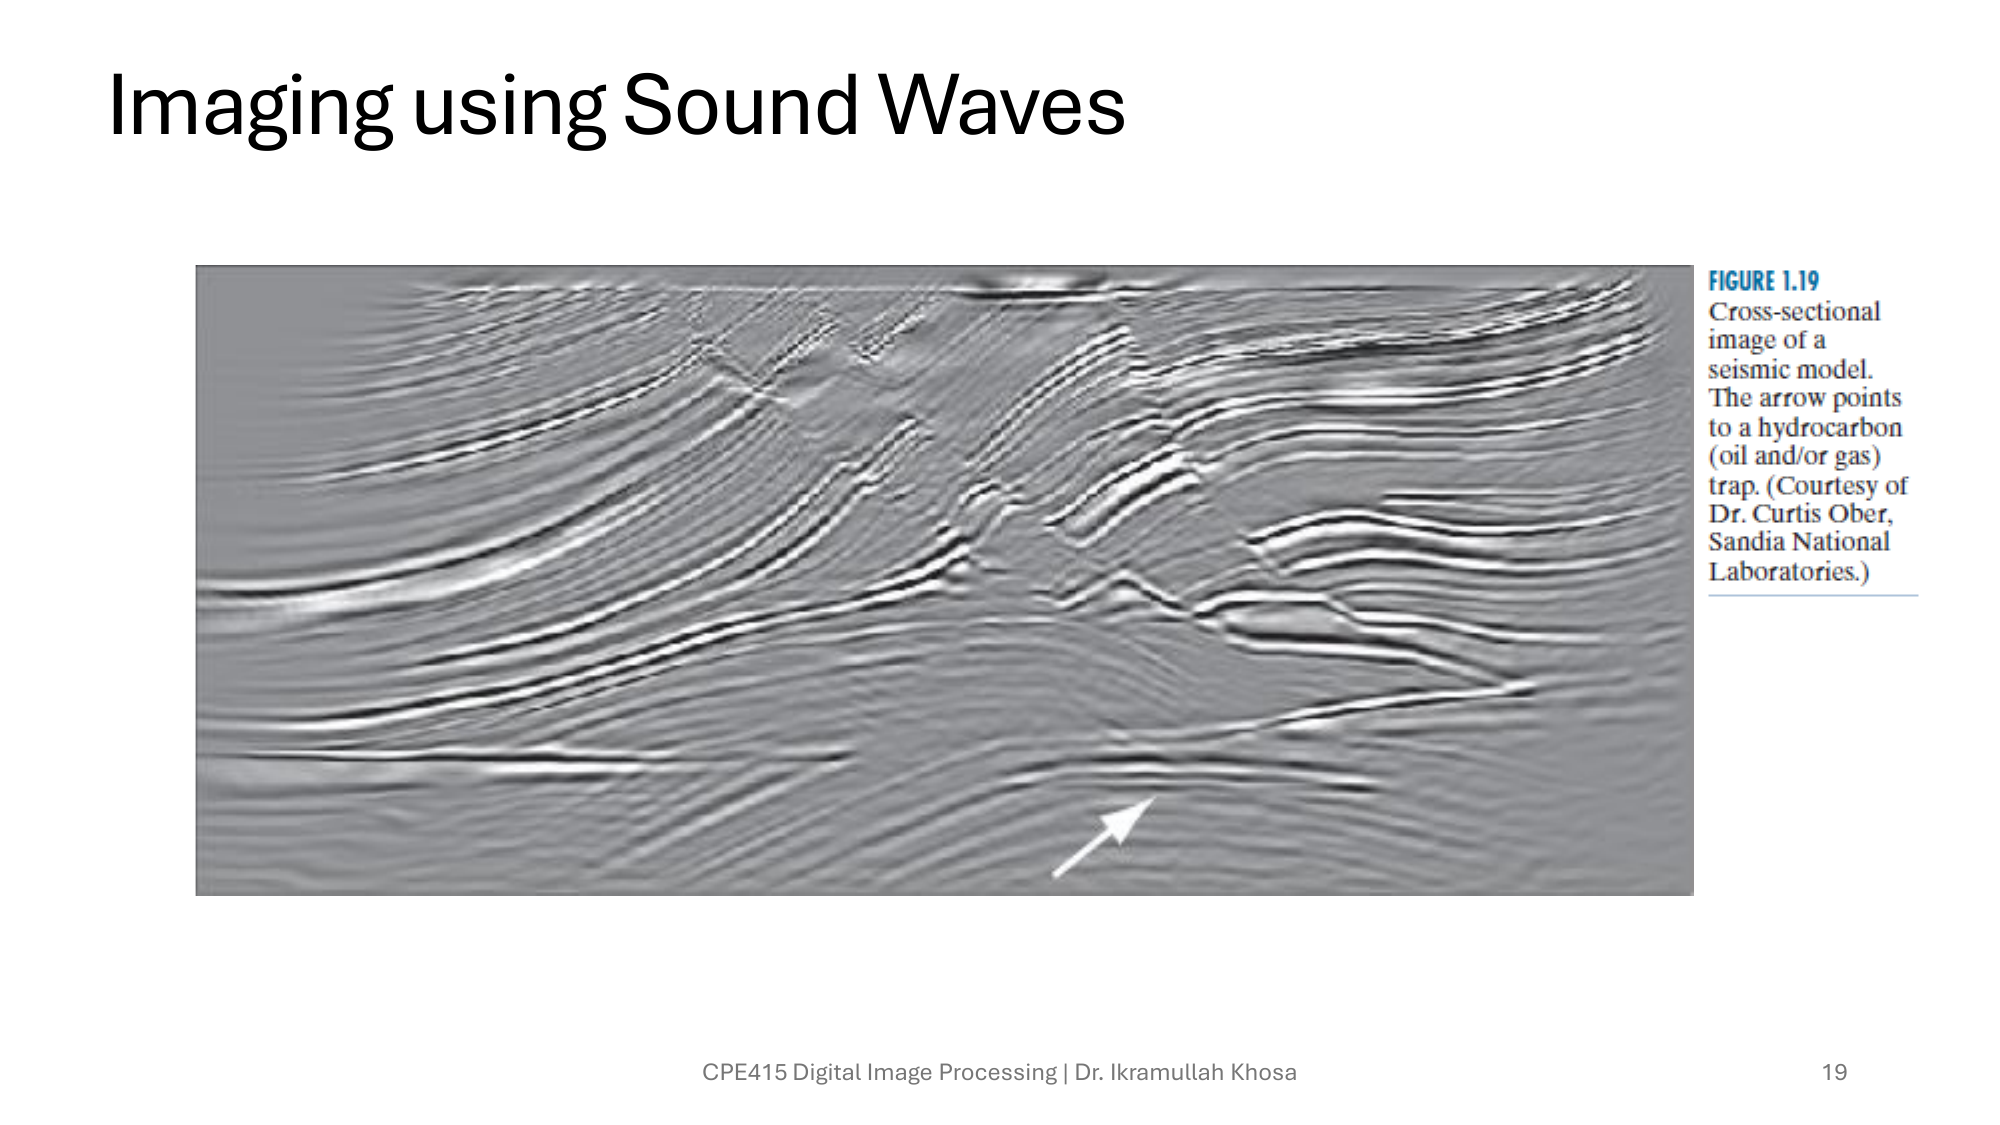
\includegraphics[width=0.9\textwidth]{images/slide1-19.png}
    \caption{Acoustic imaging using sound waves}
    \label{fig:acoustic}
\end{figure}

\begin{figure}[H]
    \centering
    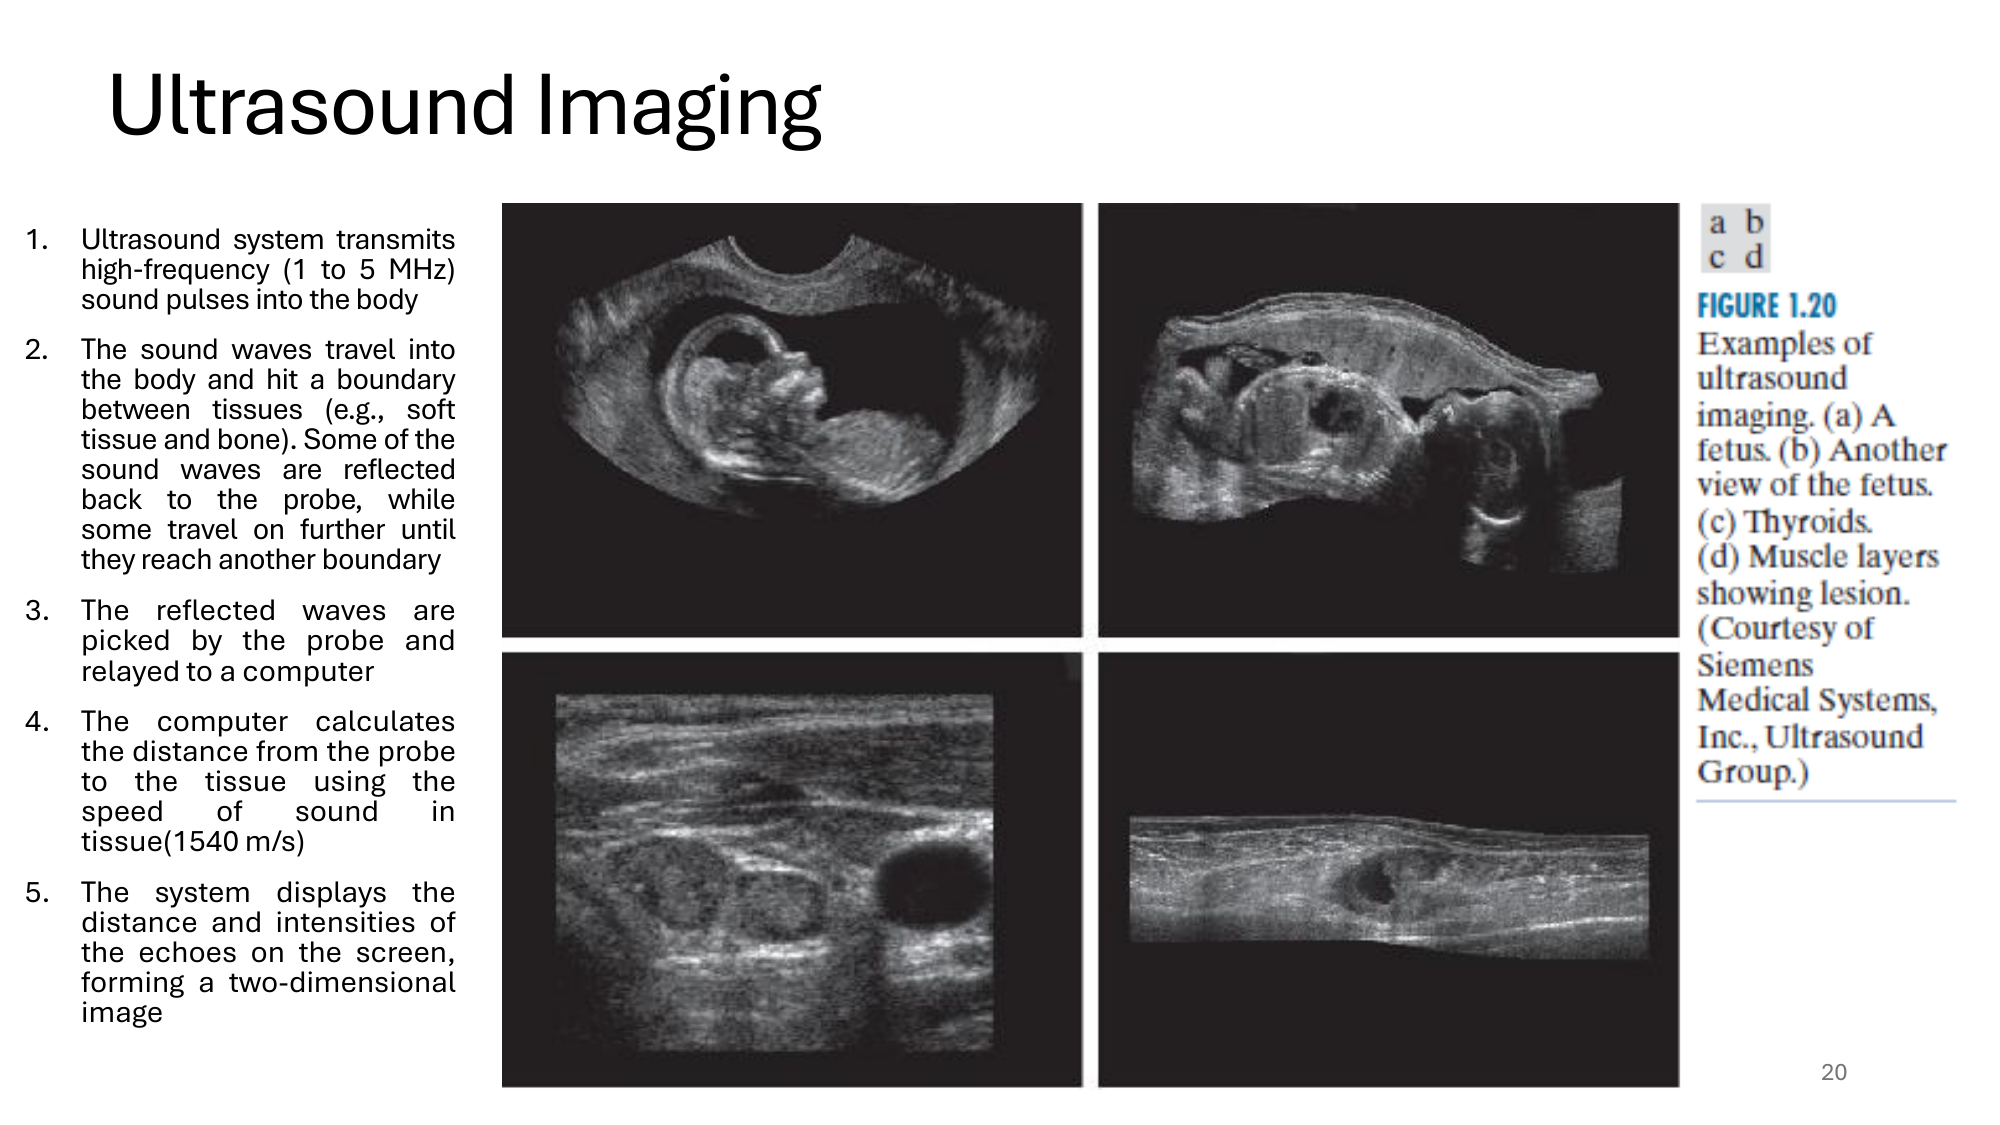
\includegraphics[width=0.9\textwidth]{images/slide1-20.png}
    \caption{Ultrasound imaging system and principles}
    \label{fig:ultrasound}
\end{figure}

\begin{deepexplanation}
\textbf{DEEP ANALYSIS - Figures \ref{fig:acoustic} and \ref{fig:ultrasound}: Ultrasound Imaging}

\textbf{The Physics:}
Ultrasound uses \textbf{mechanical waves} (not EM waves) --- high-frequency pressure oscillations.

\textbf{Typical Parameters:}
\begin{itemize}
    \item Frequency: 1--20 MHz (above human hearing: $>$ 20 kHz)
    \item Speed in tissue: $\approx 1540$ m/s (varies by tissue type)
    \item Higher frequency $\rightarrow$ better resolution but less penetration
\end{itemize}

\textbf{Image Formation Process:}
\begin{enumerate}
    \item \textbf{Transmit}: Piezoelectric transducer converts electrical pulse to sound wave
    \item \textbf{Propagate}: Sound travels into body
    \item \textbf{Reflect}: At tissue boundaries (acoustic impedance mismatch), some sound reflects
    \item \textbf{Receive}: Transducer detects returning echoes
    \item \textbf{Process}: Time delay $\rightarrow$ depth; echo amplitude $\rightarrow$ brightness
\end{enumerate}

\textbf{Distance Calculation:}
\[
d = \frac{v \cdot t}{2}
\]
where $v \approx 1540$ m/s, $t$ = round-trip time, divide by 2 for one-way distance.

\textbf{Acoustic Impedance:}
\[
Z = \rho \cdot v
\]
where $\rho$ = density, $v$ = sound velocity.

Reflection occurs at impedance boundaries:
\[
R = \left(\frac{Z_2 - Z_1}{Z_2 + Z_1}\right)^2
\]

\textbf{Why Ultrasound Is Widely Used:}
\begin{itemize}
    \item \textbf{Safe}: No ionizing radiation
    \item \textbf{Real-time}: Can see motion (heart, fetus)
    \item \textbf{Portable}: Equipment can be handheld
    \item \textbf{Inexpensive}: Compared to CT, MRI
    \item \textbf{No patient prep}: Usually no contrast needed
\end{itemize}

\textbf{Limitations:}
\begin{itemize}
    \item Cannot penetrate bone or air (strong reflection)
    \item Resolution limited by frequency/penetration trade-off
    \item Operator-dependent (probe positioning matters)
\end{itemize}
\end{deepexplanation}

\subsection{Electron Microscopy}

\begin{figure}[H]
    \centering
    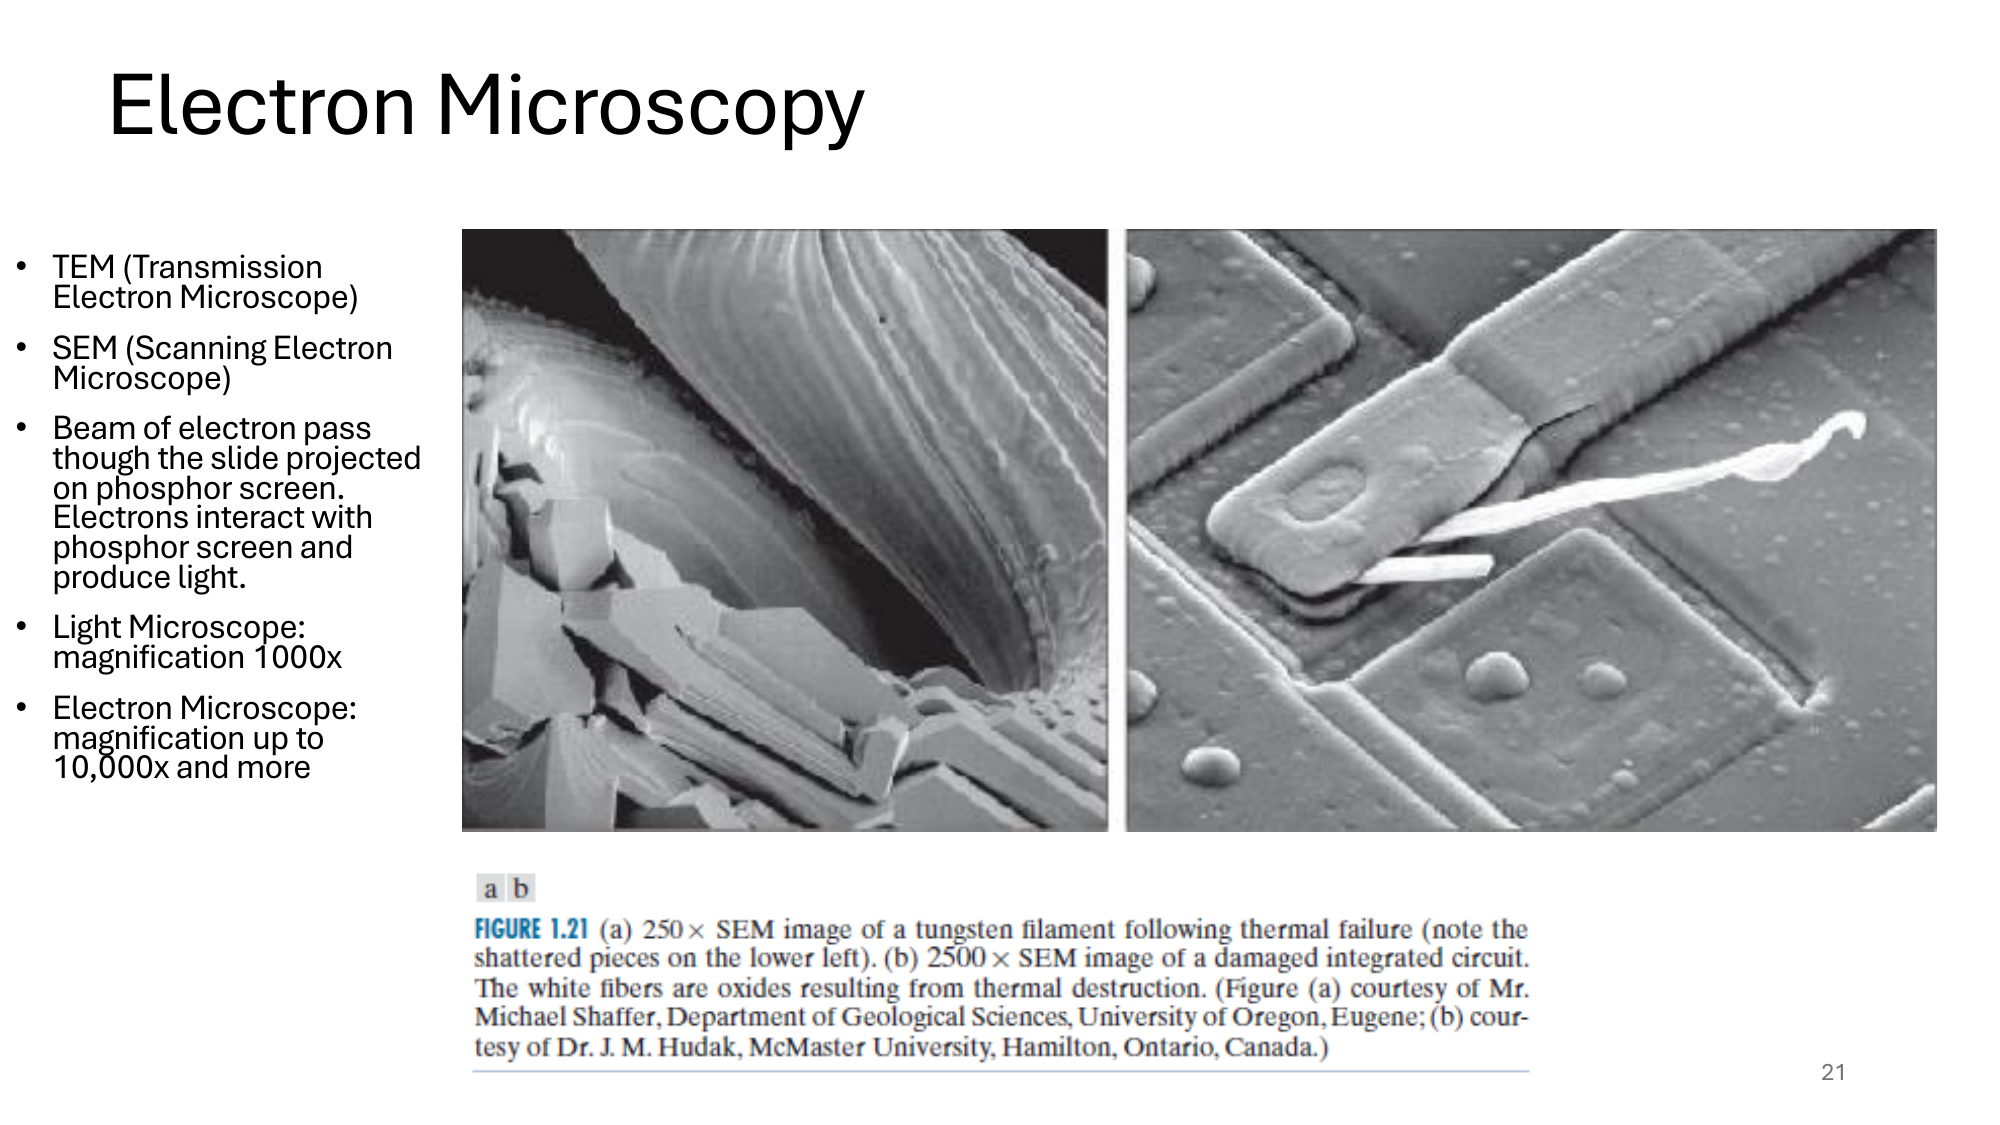
\includegraphics[width=0.9\textwidth]{images/slide1-21.png}
    \caption{Electron microscopy: TEM and SEM}
    \label{fig:electron_microscopy}
\end{figure}

\begin{deepexplanation}
\textbf{DEEP ANALYSIS - Figure \ref{fig:electron_microscopy}: Electron Microscopy}

\textbf{Why Electrons Instead of Light?}

\textbf{The Resolution Problem:}
Light microscopy is limited by diffraction:
\[
d_{min} \approx \frac{\lambda}{2}
\]
Visible light: $\lambda \approx 500$ nm $\rightarrow$ resolution limit $\approx 250$ nm.

\textbf{The Solution --- de Broglie Wavelength:}
Electrons have wave properties:
\[
\lambda = \frac{h}{p} = \frac{h}{\sqrt{2 m_e E}}
\]
At 100 keV: $\lambda \approx 0.004$ nm (much smaller than light!)

\textbf{Two Types of Electron Microscopy:}

\textbf{1. Transmission Electron Microscopy (TEM):}
\begin{itemize}
    \item Electrons pass \textbf{through} thin sample ($< 100$ nm)
    \item Analogous to optical microscope but with electrons
    \item Magnetic lenses focus electron beam
    \item Resolution: $< 0.1$ nm (can see individual atoms!)
    \item Sample must be very thin (electrons absorbed otherwise)
    \item Vacuum required (electrons scatter in air)
\end{itemize}

\textbf{2. Scanning Electron Microscopy (SEM):}
\begin{itemize}
    \item Focused electron beam scans across sample surface
    \item Detects \textbf{secondary electrons} knocked off surface
    \item Creates 3D-like surface image with great depth of field
    \item Resolution: $\approx 1$--$10$ nm
    \item Sample can be bulk (not thin)
    \item Surface must be conductive (or coated with gold/carbon)
\end{itemize}

\textbf{Magnification Comparison:}
\begin{center}
\begin{tabular}{|l|c|c|}
\hline
\textbf{Microscope} & \textbf{Max Magnification} & \textbf{Resolution} \\
\hline
Light microscope & $\approx 1000\times$ & $\approx 200$ nm \\
SEM & $\approx 500,000\times$ & $\approx 1$ nm \\
TEM & $\approx 50,000,000\times$ & $\approx 0.05$ nm \\
\hline
\end{tabular}
\end{center}

\textbf{Image Processing in EM:}
\begin{itemize}
    \item Contrast enhancement
    \item Noise reduction (low signal in biological samples)
    \item Tomographic reconstruction (3D from tilt series)
    \item Particle averaging (for single-particle analysis)
\end{itemize}
\end{deepexplanation}

%==============================================================================
\section{Computer Generated Images}
%==============================================================================

\begin{figure}[H]
    \centering
    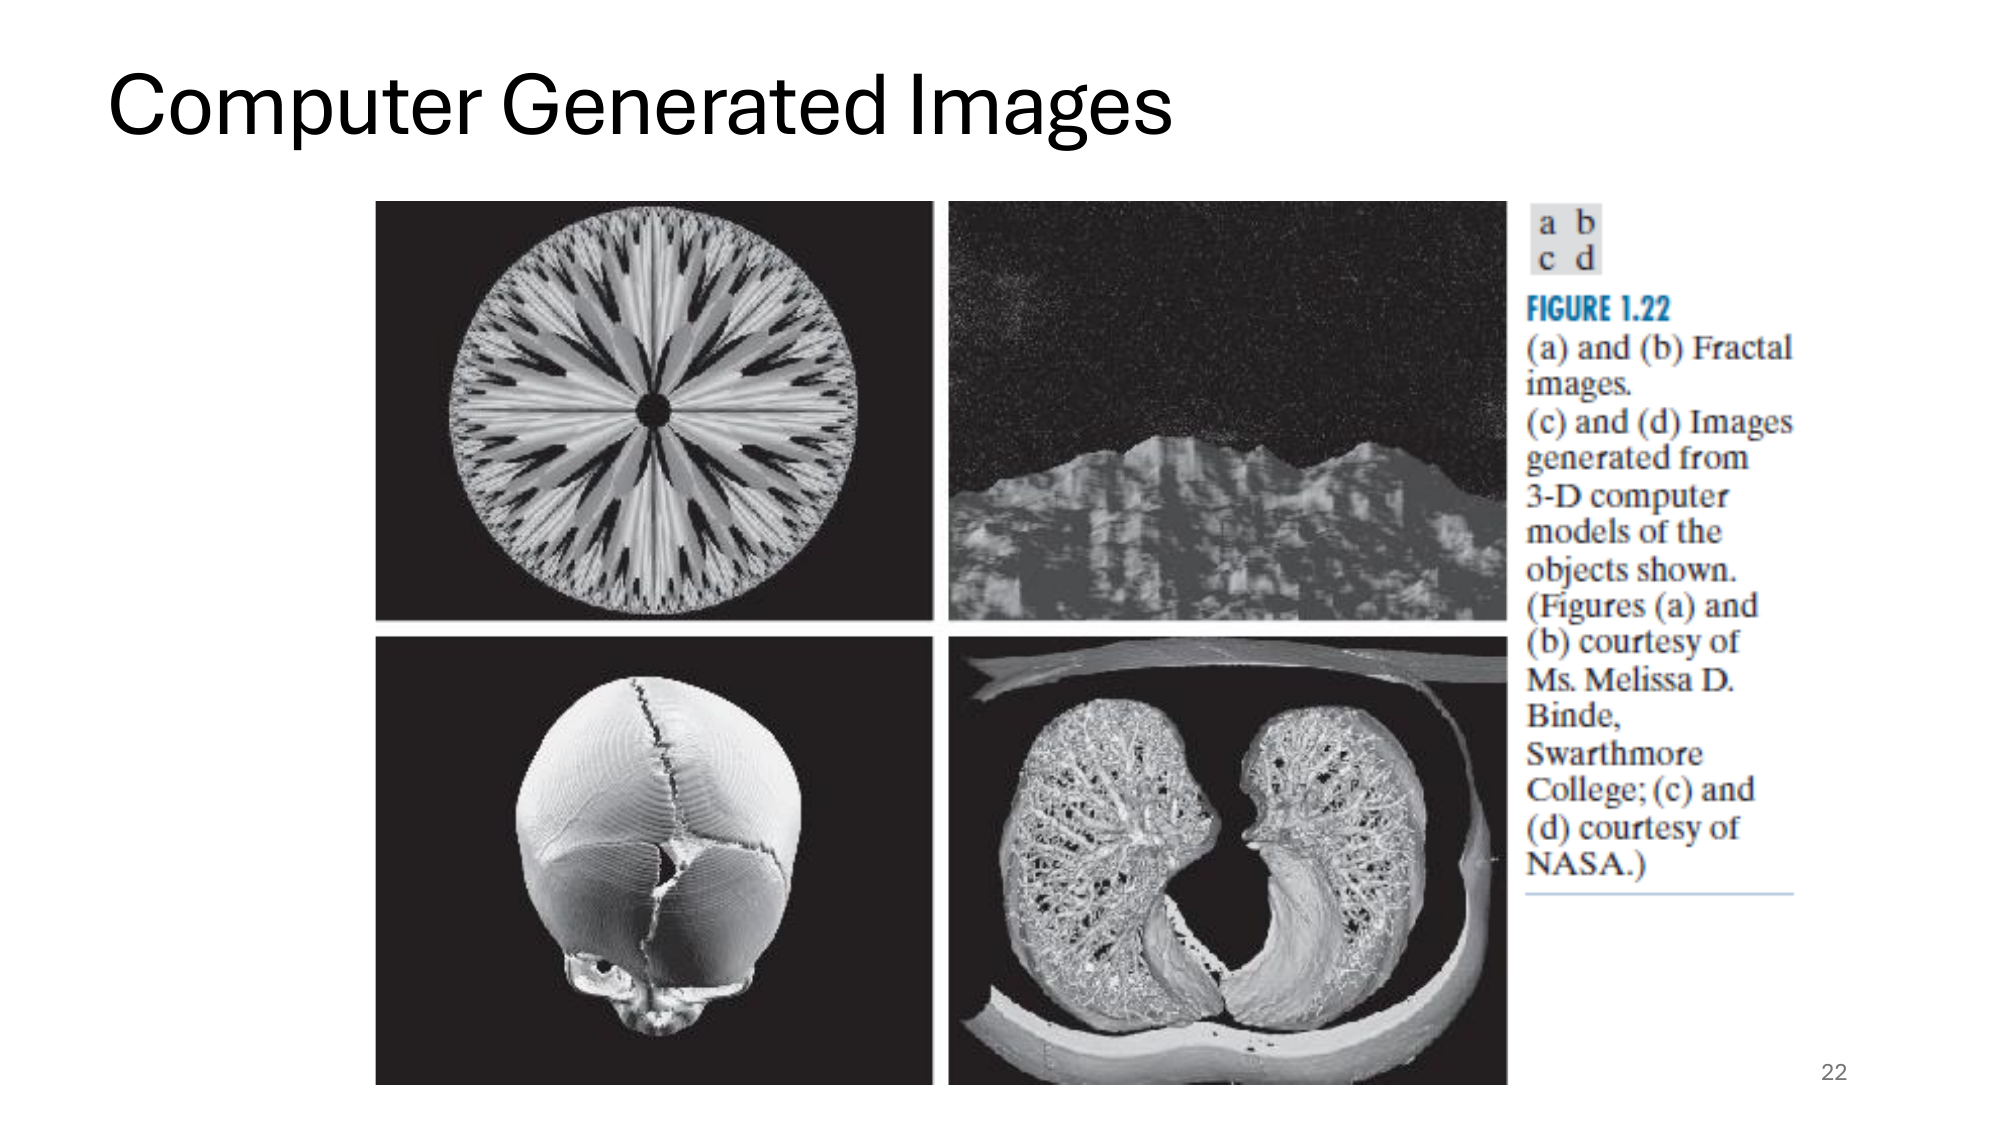
\includegraphics[width=0.9\textwidth]{images/slide1-22.png}
    \caption{Computer generated images: fractals and synthetic imagery}
    \label{fig:cgi}
\end{figure}

\begin{deepexplanation}
\textbf{DEEP ANALYSIS - Figure \ref{fig:cgi}: Synthetic and Computer-Generated Images}

\textbf{Types of Computer-Generated Images:}

\textbf{1. Mathematical/Fractal Images:}
\begin{itemize}
    \item Generated purely by mathematical formulas
    \item Example: Mandelbrot set: $z_{n+1} = z_n^2 + c$
    \item Color assigned based on iteration count
    \item Infinite detail at any zoom level
\end{itemize}

\textbf{2. 3D Rendering:}
\begin{itemize}
    \item Model scene with geometric primitives
    \item Apply materials and textures
    \item Simulate lighting and shadows
    \item Ray tracing for realistic reflections/refractions
\end{itemize}

\textbf{3. Procedural Generation:}
\begin{itemize}
    \item Algorithms create textures, terrains, objects
    \item Noise functions (Perlin noise) for natural-looking variation
    \item Used in games, movies, simulations
\end{itemize}

\textbf{Why CGI Matters for Image Processing:}
\begin{itemize}
    \item \textbf{Ground truth}: Know exactly what's in synthetic image (for testing algorithms)
    \item \textbf{Training data}: Generate labeled data for machine learning
    \item \textbf{Simulation}: Test systems before deploying on real data
    \item \textbf{Augmentation}: Expand limited datasets
\end{itemize}

\textbf{Image Processing for CGI:}
\begin{itemize}
    \item Anti-aliasing (reduce jaggies)
    \item Compositing (combine rendered elements)
    \item Post-processing effects (bloom, motion blur, depth of field)
    \item Color grading
\end{itemize}
\end{deepexplanation}


%==============================================================================
\section{Fundamental Steps in Digital Image Processing}
%==============================================================================

\begin{figure}[H]
    \centering
    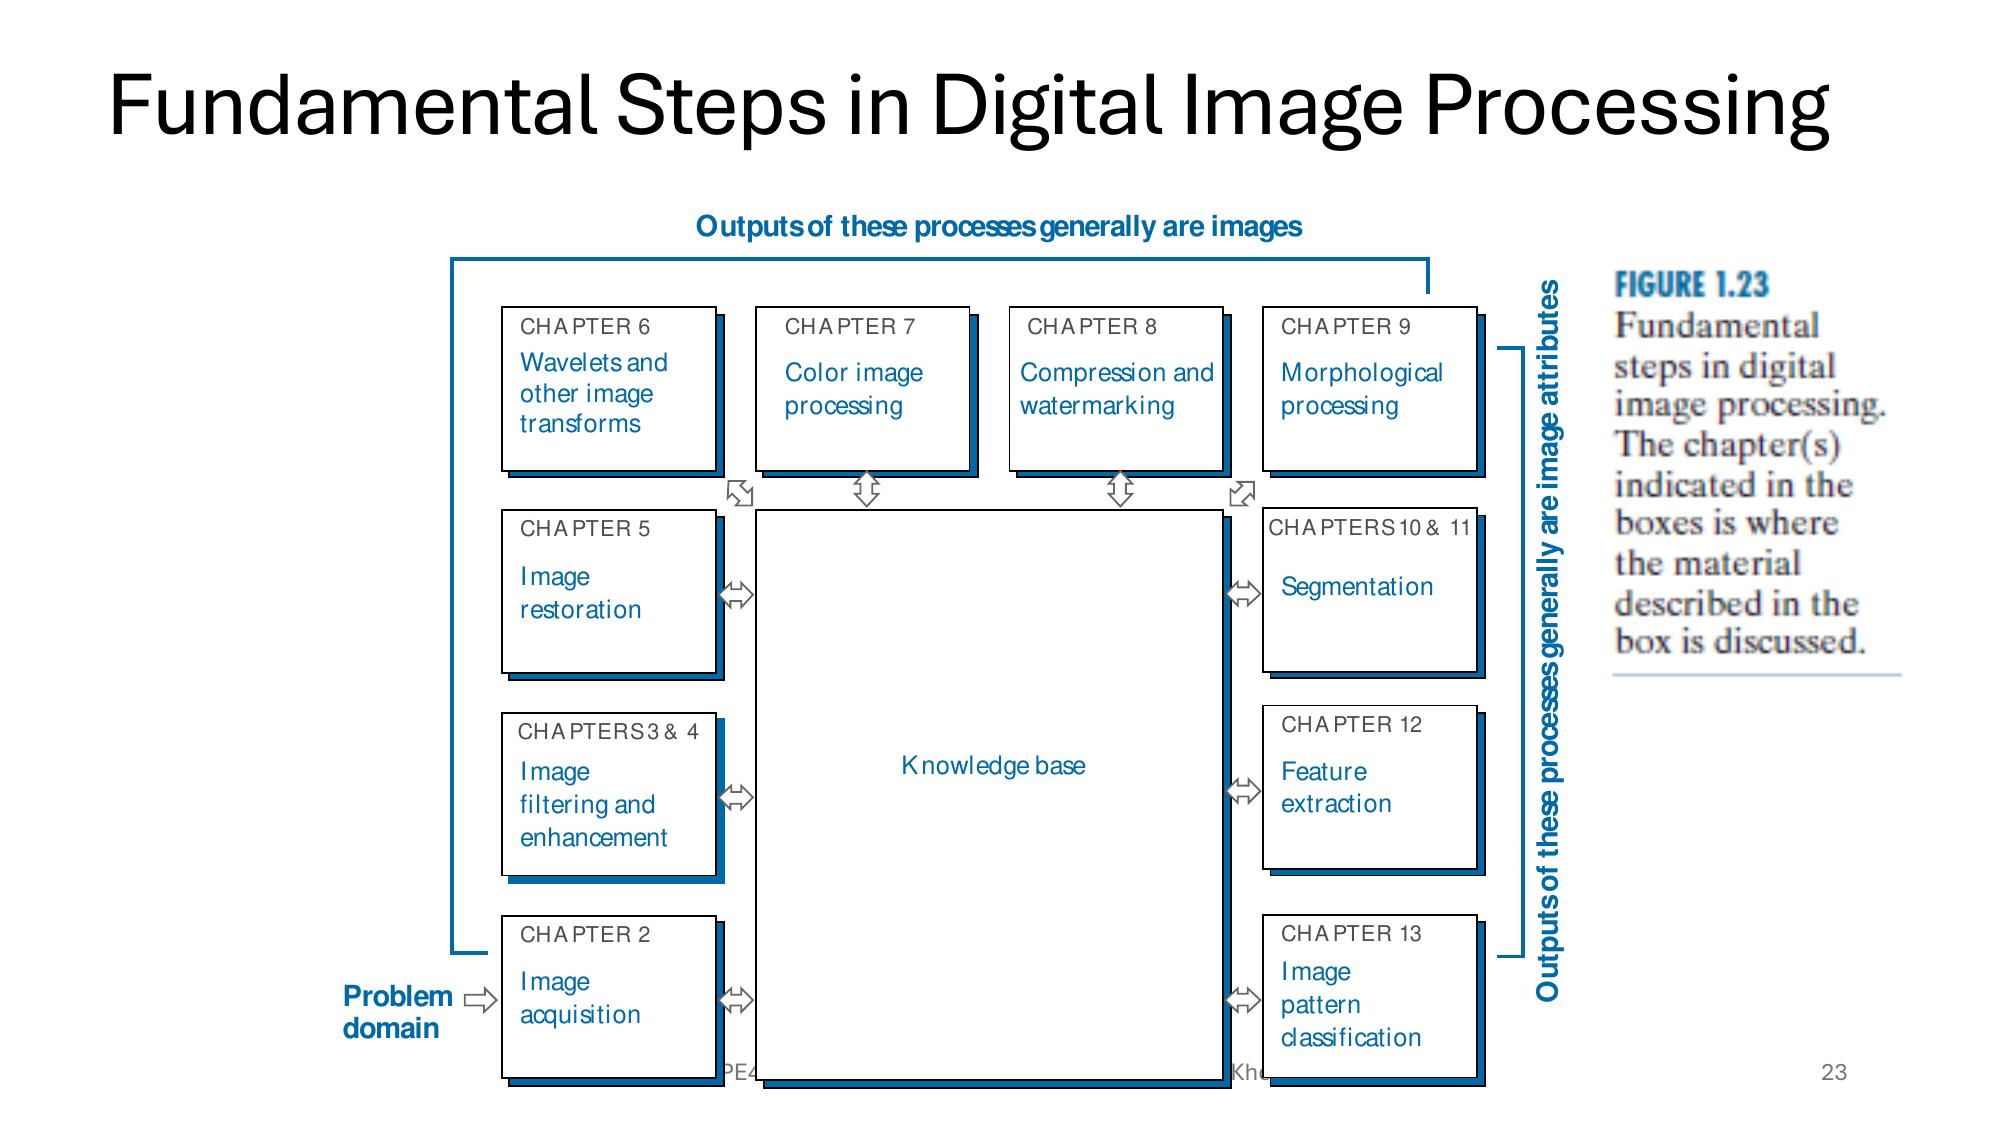
\includegraphics[width=0.95\textwidth]{images/slide1-23.png}
    \caption{Fundamental steps in digital image processing}
    \label{fig:dip_steps}
\end{figure}

\begin{deepexplanation}
\textbf{DEEP ANALYSIS - Figure \ref{fig:dip_steps}: The Image Processing Pipeline}

This diagram shows the complete chain of processing steps in a typical image processing system. Let's understand each step in detail:

\textbf{1. Image Acquisition (Chapter 2):}
\begin{itemize}
    \item Convert continuous scene to digital image
    \item Includes sensor characteristics, sampling, quantization
    \item First step --- quality here affects all subsequent steps
    \item Output: Raw digital image
\end{itemize}

\textbf{2. Image Filtering and Enhancement (Chapters 3 \& 4):}
\begin{itemize}
    \item Improve image quality for human viewing OR subsequent processing
    \item \textbf{Spatial domain}: Operate directly on pixels (contrast stretch, histogram equalization, spatial filtering)
    \item \textbf{Frequency domain}: Transform, modify spectrum, inverse transform (smoothing, sharpening, noise reduction)
    \item Output: Enhanced image
\end{itemize}

\textbf{3. Image Restoration (Chapter 5):}
\begin{itemize}
    \item Remove known degradations (blur, noise)
    \item Unlike enhancement, restoration is based on \textbf{models} of degradation
    \item Deconvolution, inverse filtering, Wiener filtering
    \item Output: Restored (de-blurred, de-noised) image
\end{itemize}

\textbf{4. Color Image Processing (Chapter 6):}
\begin{itemize}
    \item Extend grayscale techniques to color
    \item Color models: RGB, HSI, CMYK
    \item Color transformations, segmentation, enhancement
    \item Output: Processed color image
\end{itemize}

\textbf{5. Wavelets and Multi-resolution (Chapter 7):}
\begin{itemize}
    \item Represent image at multiple scales
    \item Wavelet transform for localized frequency analysis
    \item Applications: Compression, denoising, feature detection
    \item Output: Multi-scale representation or processed image
\end{itemize}

\textbf{6. Compression and Watermarking (Chapter 8):}
\begin{itemize}
    \item Reduce storage/transmission requirements
    \item Lossless vs lossy compression
    \item Watermarking: Embed invisible information
    \item Output: Compressed image or watermarked image
\end{itemize}

\textbf{7. Morphological Processing (Chapter 9):}
\begin{itemize}
    \item Operations based on shape
    \item Erosion, dilation, opening, closing
    \item Useful for binary images and shape analysis
    \item Output: Morphologically processed image
\end{itemize}

\textbf{8. Segmentation (Chapters 10 \& 11):}
\begin{itemize}
    \item Partition image into meaningful regions
    \item Edge detection, region growing, thresholding
    \item Critical step for object recognition
    \item Output: Segmented image (labeled regions)
\end{itemize}

\textbf{9. Feature Extraction (Chapter 12):}
\begin{itemize}
    \item Measure properties of segmented regions
    \item Shape descriptors: area, perimeter, moments
    \item Texture descriptors: statistical, structural
    \item Output: Feature vectors
\end{itemize}

\textbf{10. Classification/Recognition (Chapter 13):}
\begin{itemize}
    \item Assign labels based on features
    \item Pattern recognition, machine learning
    \item The goal of many image processing applications
    \item Output: Classification decision
\end{itemize}

\textbf{The Knowledge Base:}
Runs alongside all steps, containing:
\begin{itemize}
    \item Prior knowledge about the problem domain
    \item Constraints and expectations
    \item Training data and learned models
\end{itemize}
\end{deepexplanation}

\begin{mathbox}
\textbf{Two Categories of Output:}

\textbf{Image-to-Image:} Steps 1--8 typically output images
\begin{itemize}
    \item Acquisition $\rightarrow$ digital image
    \item Enhancement $\rightarrow$ enhanced image
    \item Restoration $\rightarrow$ restored image
    \item Compression $\rightarrow$ (encoded then decoded) image
\end{itemize}

\textbf{Image-to-Attributes:} Steps 9--10 output non-image data
\begin{itemize}
    \item Feature extraction $\rightarrow$ measurements, descriptors
    \item Classification $\rightarrow$ labels, decisions
\end{itemize}
\end{mathbox}

%==============================================================================
\section{Components of a Digital Image Processing System}
%==============================================================================

\begin{figure}[H]
    \centering
    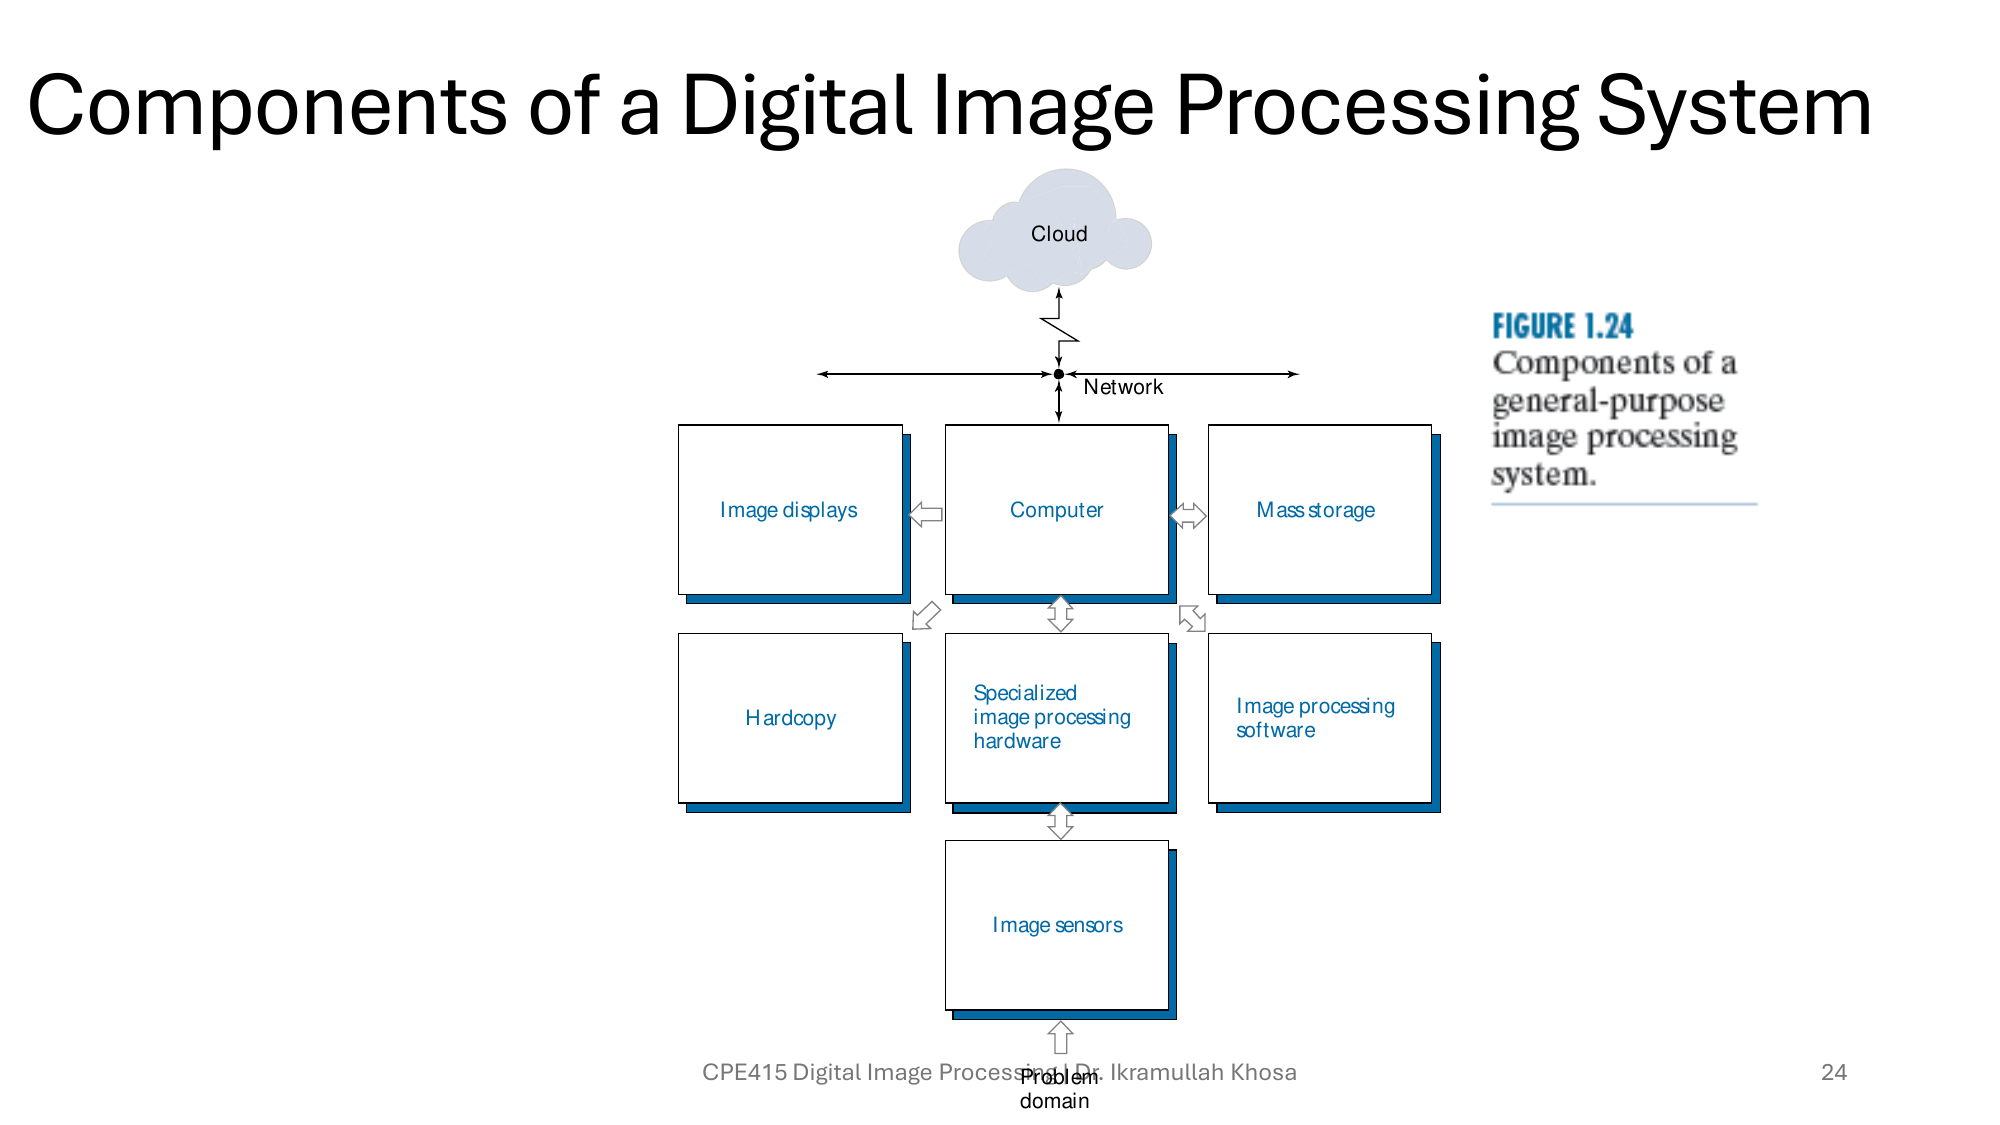
\includegraphics[width=0.95\textwidth]{images/slide1-24.png}
    \caption{Components of a digital image processing system}
    \label{fig:dip_system}
\end{figure}

\begin{deepexplanation}
\textbf{DEEP ANALYSIS - Figure \ref{fig:dip_system}: Hardware and Software Components}

\textbf{1. Image Sensors:}
\begin{itemize}
    \item Convert light (or other energy) to electrical signals
    \item Types: CCD, CMOS, thermal, X-ray detectors
    \item Key parameters: Resolution, sensitivity, dynamic range, noise
    \item Include optics (lenses) for focusing
\end{itemize}

\textbf{2. Specialized Image Processing Hardware:}
\begin{itemize}
    \item \textbf{Frame grabber}: Digitizes analog video signals
    \item \textbf{GPU (Graphics Processing Unit)}: Massive parallelism for image operations
    \item \textbf{FPGA}: Field-programmable gate array for real-time processing
    \item \textbf{DSP}: Digital signal processor for embedded systems
    \item Why specialized hardware? Images are large; many operations are highly parallel
\end{itemize}

\textbf{3. Computer (CPU/Memory):}
\begin{itemize}
    \item General-purpose processing
    \item Controls overall system
    \item Runs software algorithms
    \item Modern CPUs have SIMD instructions for image processing (SSE, AVX)
\end{itemize}

\textbf{4. Image Processing Software:}
\begin{itemize}
    \item \textbf{Libraries}: OpenCV, PIL/Pillow, scikit-image
    \item \textbf{Development environments}: MATLAB, Python, C++
    \item \textbf{Specialized packages}: Medical (ITK), remote sensing (GDAL)
    \item Implements all algorithms from acquisition to recognition
\end{itemize}

\textbf{5. Mass Storage:}
\begin{itemize}
    \item Images require significant storage
    \item Example: 1 megapixel RGB image = 3 MB uncompressed
    \item Need fast access for real-time processing
    \item Types: SSD, HDD, network storage (NAS/SAN), cloud storage
\end{itemize}

\textbf{6. Image Displays:}
\begin{itemize}
    \item LCD, OLED monitors for viewing
    \item Calibrated displays for medical, color-critical work
    \item High resolution for detail examination
    \item Multiple monitors common in professional settings
\end{itemize}

\textbf{7. Hardcopy Devices:}
\begin{itemize}
    \item Printers for physical output
    \item Film recorders (medical)
    \item Important: Print resolution differs from screen resolution
\end{itemize}

\textbf{8. Network/Cloud:}
\begin{itemize}
    \item Distribute processing across machines
    \item Access remote databases
    \item Cloud processing for intensive computations
    \item Enables collaboration and large-scale analysis
\end{itemize}
\end{deepexplanation}

%==============================================================================
\section{Applications of Digital Image Processing}
%==============================================================================

\begin{conceptbox}[Where Is Image Processing Used?]
Digital image processing touches virtually every aspect of modern technology:
\begin{itemize}
    \item \textbf{Medicine}: Diagnosis, treatment planning, surgery guidance
    \item \textbf{Remote Sensing}: Earth observation, weather, agriculture
    \item \textbf{Astronomy}: Capturing and analyzing celestial objects
    \item \textbf{Industry}: Quality control, automation, robotics
    \item \textbf{Security}: Surveillance, biometrics, forensics
    \item \textbf{Entertainment}: Photography, video, gaming, movies
    \item \textbf{Communication}: Video conferencing, compression, transmission
    \item \textbf{Scientific Research}: Biology, physics, chemistry, materials
\end{itemize}
\end{conceptbox}

\subsection{Medical Imaging Applications}

\begin{examplebox}[Medical Image Processing Examples]
\textbf{Diagnostic Imaging:}
\begin{itemize}
    \item CT: Detect tumors, internal injuries, bone fractures
    \item MRI: Soft tissue detail, brain imaging, joint problems
    \item X-ray: Chest screening, dental, bone alignment
    \item Ultrasound: Pregnancy, cardiac, abdominal organs
\end{itemize}

\textbf{Image Processing Tasks:}
\begin{itemize}
    \item Enhancement: Improve visibility of subtle features
    \item Segmentation: Identify organs, tumors, vessels
    \item Registration: Align images from different times/modalities
    \item Measurement: Quantify tumor size, bone density
    \item Computer-aided detection (CAD): Flag suspicious regions
\end{itemize}
\end{examplebox}

\subsection{Remote Sensing Applications}

\begin{examplebox}[Remote Sensing Image Processing]
\textbf{Earth Observation:}
\begin{itemize}
    \item Land use classification (urban, forest, water, agriculture)
    \item Change detection (deforestation, urbanization)
    \item Disaster assessment (floods, fires, earthquakes)
    \item Weather forecasting (cloud patterns, storm tracking)
\end{itemize}

\textbf{Image Processing Tasks:}
\begin{itemize}
    \item Atmospheric correction: Remove haze, clouds
    \item Geometric correction: Remove distortions from sensor/terrain
    \item Band combination: Create false-color composites
    \item Classification: Identify land cover types
    \item Time series analysis: Monitor changes over time
\end{itemize}
\end{examplebox}

\subsection{Industrial and Automation Applications}

\begin{examplebox}[Machine Vision in Industry]
\textbf{Manufacturing:}
\begin{itemize}
    \item Defect detection: Scratches, cracks, missing components
    \item Dimensional measurement: Verify part sizes
    \item Assembly verification: Check correct component placement
    \item Color/texture inspection: Ensure consistency
\end{itemize}

\textbf{Automation:}
\begin{itemize}
    \item Robot guidance: Pick-and-place, welding
    \item Autonomous vehicles: Object detection, lane following
    \item Barcode/QR reading: Logistics, inventory
    \item OCR: Document processing, mail sorting
\end{itemize}

\textbf{Image Processing Tasks:}
\begin{itemize}
    \item High-speed processing (real-time)
    \item Precise edge detection
    \item Pattern matching
    \item Calibration and measurement
\end{itemize}
\end{examplebox}

%==============================================================================
\section{The Mathematical Foundation}
%==============================================================================

\subsection{Images as Functions}

\begin{mathbox}
\textbf{The 2D Continuous Image:}
\[
f(x, y) : \mathbb{R}^2 \rightarrow \mathbb{R}^+
\]
\begin{itemize}
    \item Domain: Continuous spatial coordinates $(x, y)$
    \item Range: Non-negative real values (intensity)
    \item Color images: Vector-valued $\vec{f}(x,y) = [R(x,y), G(x,y), B(x,y)]^T$
\end{itemize}

\textbf{The 2D Digital Image:}
\[
f[m, n] : \mathbb{Z}^2 \rightarrow \{0, 1, 2, \ldots, L-1\}
\]
\begin{itemize}
    \item Domain: Integer coordinates $m \in \{0, \ldots, M-1\}$, $n \in \{0, \ldots, N-1\}$
    \item Range: Finite set of $L$ gray levels (typically $L = 256$ for 8-bit)
\end{itemize}
\end{mathbox}

\subsection{Image Processing Operations}

\begin{conceptbox}[Types of Image Operations]
\textbf{1. Point Operations (Pixel-wise):}
\[
g(x, y) = T[f(x, y)]
\]
Output depends only on input value at that location.
Examples: Brightness adjustment, contrast stretch, thresholding.

\textbf{2. Neighborhood Operations (Local):}
\[
g(x, y) = T[f(x-k, y-l)] \text{ for } (k, l) \in \mathcal{N}
\]
Output depends on pixel and its neighbors.
Examples: Smoothing, sharpening, edge detection.

\textbf{3. Global Operations:}
\[
g(x, y) = T[f(u, v)] \text{ for all } (u, v)
\]
Output depends on entire image.
Examples: Fourier transform, histogram equalization.
\end{conceptbox}

%==============================================================================
\section{Summary and Roadmap}
%==============================================================================

\begin{importantbox}
\textbf{Key Takeaways from Chapter 1:}

\begin{enumerate}
    \item \textbf{Definition}: A digital image is a 2D array of discrete intensity values at discrete spatial locations.
    
    \item \textbf{Versatility}: Images can be formed from the entire EM spectrum plus acoustic and other energy sources.
    
    \item \textbf{Rich Information}: Different wavelengths/modalities reveal different information about the same scene.
    
    \item \textbf{Processing Pipeline}: Image processing involves a chain of steps from acquisition through enhancement, restoration, segmentation, to recognition.
    
    \item \textbf{Hardware + Software}: Modern systems combine specialized hardware with sophisticated algorithms.
    
    \item \textbf{Ubiquitous Applications}: From medicine to astronomy to entertainment, image processing is everywhere.
\end{enumerate}
\end{importantbox}

\subsection{Course Roadmap}

\begin{conceptbox}[What's Ahead]
\textbf{Chapter 2: Digital Image Fundamentals}
\begin{itemize}
    \item Human visual system
    \item Sampling and quantization
    \item Pixel relationships
    \item Basic operations
\end{itemize}

\textbf{Chapter 3: Intensity Transformations and Spatial Filtering}
\begin{itemize}
    \item Point operations (histogram, contrast)
    \item Convolution and spatial filters
    \item Smoothing and sharpening
\end{itemize}

\textbf{Chapter 4: Frequency Domain Filtering}
\begin{itemize}
    \item Fourier transform
    \item Low-pass and high-pass filtering
    \item Filtering in frequency domain
\end{itemize}

\textbf{And beyond}: Restoration, color, wavelets, compression, morphology, segmentation, features, recognition...
\end{conceptbox}

%==============================================================================
\section{Review Questions}
%==============================================================================

\begin{examplebox}[Self-Assessment]
\textbf{Conceptual Questions:}
\begin{enumerate}
    \item What distinguishes a digital image from an analog image?
    
    \item Why can different EM wavelengths reveal different information about the same scene?
    
    \item Explain why MRI uses radio waves but can image internal body structures.
    
    \item What is the fundamental resolution limit of light microscopy, and how do electron microscopes overcome it?
    
    \item Describe the difference between image enhancement and image restoration.
\end{enumerate}

\textbf{Application Questions:}
\begin{enumerate}
    \item Which imaging modality would you use to:
    \begin{itemize}
        \item Detect a brain tumor? (MRI --- excellent soft tissue contrast)
        \item Map crop health over a large farm? (Multispectral satellite --- NDVI)
        \item Inspect circuit boards for defects? (Visible light machine vision)
        \item Find hot spots in electrical equipment? (Thermal IR)
    \end{itemize}
    
    \item Why does CT use X-rays while MRI uses radio waves?
    
    \item What advantages does SAR have over optical satellite imaging?
\end{enumerate}
\end{examplebox}

\end{document}
